% Options for packages loaded elsewhere
\PassOptionsToPackage{unicode}{hyperref}
\PassOptionsToPackage{hyphens}{url}
\PassOptionsToPackage{dvipsnames,svgnames,x11names}{xcolor}
%
\documentclass[
]{article}

\usepackage{amsmath,amssymb}
\usepackage{iftex}
\ifPDFTeX
  \usepackage[T1]{fontenc}
  \usepackage[utf8]{inputenc}
  \usepackage{textcomp} % provide euro and other symbols
\else % if luatex or xetex
  \usepackage{unicode-math}
  \defaultfontfeatures{Scale=MatchLowercase}
  \defaultfontfeatures[\rmfamily]{Ligatures=TeX,Scale=1}
\fi
\usepackage{lmodern}
\ifPDFTeX\else  
    % xetex/luatex font selection
\fi
% Use upquote if available, for straight quotes in verbatim environments
\IfFileExists{upquote.sty}{\usepackage{upquote}}{}
\IfFileExists{microtype.sty}{% use microtype if available
  \usepackage[]{microtype}
  \UseMicrotypeSet[protrusion]{basicmath} % disable protrusion for tt fonts
}{}
\makeatletter
\@ifundefined{KOMAClassName}{% if non-KOMA class
  \IfFileExists{parskip.sty}{%
    \usepackage{parskip}
  }{% else
    \setlength{\parindent}{0pt}
    \setlength{\parskip}{6pt plus 2pt minus 1pt}}
}{% if KOMA class
  \KOMAoptions{parskip=half}}
\makeatother
\usepackage{xcolor}
\setlength{\emergencystretch}{3em} % prevent overfull lines
\setcounter{secnumdepth}{5}
% Make \paragraph and \subparagraph free-standing
\ifx\paragraph\undefined\else
  \let\oldparagraph\paragraph
  \renewcommand{\paragraph}[1]{\oldparagraph{#1}\mbox{}}
\fi
\ifx\subparagraph\undefined\else
  \let\oldsubparagraph\subparagraph
  \renewcommand{\subparagraph}[1]{\oldsubparagraph{#1}\mbox{}}
\fi

\usepackage{color}
\usepackage{fancyvrb}
\newcommand{\VerbBar}{|}
\newcommand{\VERB}{\Verb[commandchars=\\\{\}]}
\DefineVerbatimEnvironment{Highlighting}{Verbatim}{commandchars=\\\{\}}
% Add ',fontsize=\small' for more characters per line
\usepackage{framed}
\definecolor{shadecolor}{RGB}{248,248,248}
\newenvironment{Shaded}{\begin{snugshade}}{\end{snugshade}}
\newcommand{\AlertTok}[1]{\textcolor[rgb]{0.94,0.16,0.16}{#1}}
\newcommand{\AnnotationTok}[1]{\textcolor[rgb]{0.56,0.35,0.01}{\textbf{\textit{#1}}}}
\newcommand{\AttributeTok}[1]{\textcolor[rgb]{0.77,0.63,0.00}{#1}}
\newcommand{\BaseNTok}[1]{\textcolor[rgb]{0.00,0.00,0.81}{#1}}
\newcommand{\BuiltInTok}[1]{\textcolor[rgb]{0.00,0.00,0.00}{#1}}
\newcommand{\CharTok}[1]{\textcolor[rgb]{0.31,0.60,0.02}{#1}}
\newcommand{\CommentTok}[1]{\textcolor[rgb]{0.56,0.35,0.01}{\textit{#1}}}
\newcommand{\CommentVarTok}[1]{\textcolor[rgb]{0.56,0.35,0.01}{\textbf{\textit{#1}}}}
\newcommand{\ConstantTok}[1]{\textcolor[rgb]{0.00,0.00,0.00}{#1}}
\newcommand{\ControlFlowTok}[1]{\textcolor[rgb]{0.13,0.29,0.53}{\textbf{#1}}}
\newcommand{\DataTypeTok}[1]{\textcolor[rgb]{0.13,0.29,0.53}{#1}}
\newcommand{\DecValTok}[1]{\textcolor[rgb]{0.00,0.00,0.81}{#1}}
\newcommand{\DocumentationTok}[1]{\textcolor[rgb]{0.56,0.35,0.01}{\textbf{\textit{#1}}}}
\newcommand{\ErrorTok}[1]{\textcolor[rgb]{0.64,0.00,0.00}{\textbf{#1}}}
\newcommand{\ExtensionTok}[1]{\textcolor[rgb]{0.00,0.00,0.00}{#1}}
\newcommand{\FloatTok}[1]{\textcolor[rgb]{0.00,0.00,0.81}{#1}}
\newcommand{\FunctionTok}[1]{\textcolor[rgb]{0.00,0.00,0.00}{#1}}
\newcommand{\ImportTok}[1]{\textcolor[rgb]{0.00,0.00,0.00}{#1}}
\newcommand{\InformationTok}[1]{\textcolor[rgb]{0.56,0.35,0.01}{\textbf{\textit{#1}}}}
\newcommand{\KeywordTok}[1]{\textcolor[rgb]{0.13,0.29,0.53}{\textbf{#1}}}
\newcommand{\NormalTok}[1]{\textcolor[rgb]{0.00,0.00,0.00}{#1}}
\newcommand{\OperatorTok}[1]{\textcolor[rgb]{0.81,0.36,0.00}{\textbf{#1}}}
\newcommand{\OtherTok}[1]{\textcolor[rgb]{0.56,0.35,0.01}{#1}}
\newcommand{\PreprocessorTok}[1]{\textcolor[rgb]{0.56,0.35,0.01}{\textit{#1}}}
\newcommand{\RegionMarkerTok}[1]{\textcolor[rgb]{0.00,0.00,0.00}{#1}}
\newcommand{\SpecialCharTok}[1]{\textcolor[rgb]{0.00,0.00,0.00}{#1}}
\newcommand{\SpecialStringTok}[1]{\textcolor[rgb]{0.31,0.60,0.02}{#1}}
\newcommand{\StringTok}[1]{\textcolor[rgb]{0.31,0.60,0.02}{#1}}
\newcommand{\VariableTok}[1]{\textcolor[rgb]{0.00,0.00,0.00}{#1}}
\newcommand{\VerbatimStringTok}[1]{\textcolor[rgb]{0.31,0.60,0.02}{#1}}
\newcommand{\WarningTok}[1]{\textcolor[rgb]{0.56,0.35,0.01}{\textbf{\textit{#1}}}}

\providecommand{\tightlist}{%
  \setlength{\itemsep}{0pt}\setlength{\parskip}{0pt}}\usepackage{longtable,booktabs,array}
\usepackage{calc} % for calculating minipage widths
% Correct order of tables after \paragraph or \subparagraph
\usepackage{etoolbox}
\makeatletter
\patchcmd\longtable{\par}{\if@noskipsec\mbox{}\fi\par}{}{}
\makeatother
% Allow footnotes in longtable head/foot
\IfFileExists{footnotehyper.sty}{\usepackage{footnotehyper}}{\usepackage{footnote}}
\makesavenoteenv{longtable}
\usepackage{graphicx}
\makeatletter
\def\maxwidth{\ifdim\Gin@nat@width>\linewidth\linewidth\else\Gin@nat@width\fi}
\def\maxheight{\ifdim\Gin@nat@height>\textheight\textheight\else\Gin@nat@height\fi}
\makeatother
% Scale images if necessary, so that they will not overflow the page
% margins by default, and it is still possible to overwrite the defaults
% using explicit options in \includegraphics[width, height, ...]{}
\setkeys{Gin}{width=\maxwidth,height=\maxheight,keepaspectratio}
% Set default figure placement to htbp
\makeatletter
\def\fps@figure{htbp}
\makeatother

\makeatletter
\makeatother
\makeatletter
\makeatother
\makeatletter
\@ifpackageloaded{caption}{}{\usepackage{caption}}
\AtBeginDocument{%
\ifdefined\contentsname
  \renewcommand*\contentsname{Table of contents}
\else
  \newcommand\contentsname{Table of contents}
\fi
\ifdefined\listfigurename
  \renewcommand*\listfigurename{List of Figures}
\else
  \newcommand\listfigurename{List of Figures}
\fi
\ifdefined\listtablename
  \renewcommand*\listtablename{List of Tables}
\else
  \newcommand\listtablename{List of Tables}
\fi
\ifdefined\figurename
  \renewcommand*\figurename{Figure}
\else
  \newcommand\figurename{Figure}
\fi
\ifdefined\tablename
  \renewcommand*\tablename{Table}
\else
  \newcommand\tablename{Table}
\fi
}
\@ifpackageloaded{float}{}{\usepackage{float}}
\floatstyle{ruled}
\@ifundefined{c@chapter}{\newfloat{codelisting}{h}{lop}}{\newfloat{codelisting}{h}{lop}[chapter]}
\floatname{codelisting}{Listing}
\newcommand*\listoflistings{\listof{codelisting}{List of Listings}}
\makeatother
\makeatletter
\@ifpackageloaded{caption}{}{\usepackage{caption}}
\@ifpackageloaded{subcaption}{}{\usepackage{subcaption}}
\makeatother
\makeatletter
\makeatother
\ifLuaTeX
  \usepackage{selnolig}  % disable illegal ligatures
\fi
\IfFileExists{bookmark.sty}{\usepackage{bookmark}}{\usepackage{hyperref}}
\IfFileExists{xurl.sty}{\usepackage{xurl}}{} % add URL line breaks if available
\urlstyle{same} % disable monospaced font for URLs
\hypersetup{
  pdftitle={Biostat 203B Homework 3},
  pdfauthor={Wenqiang Ge UID:106371961},
  colorlinks=true,
  linkcolor={blue},
  filecolor={Maroon},
  citecolor={Blue},
  urlcolor={Blue},
  pdfcreator={LaTeX via pandoc}}

\title{Biostat 203B Homework 3}
\usepackage{etoolbox}
\makeatletter
\providecommand{\subtitle}[1]{% add subtitle to \maketitle
  \apptocmd{\@title}{\par {\large #1 \par}}{}{}
}
\makeatother
\subtitle{Due Feb 21 @ 11:59PM}
\author{Wenqiang Ge UID:106371961}
\date{}

\begin{document}
\maketitle
\renewcommand*\contentsname{Table of contents}
{
\hypersetup{linkcolor=}
\setcounter{tocdepth}{2}
\tableofcontents
}
Display machine information for reproducibility:

\begin{Shaded}
\begin{Highlighting}[]
\FunctionTok{sessionInfo}\NormalTok{()}
\end{Highlighting}
\end{Shaded}

\begin{verbatim}
R version 4.4.2 (2024-10-31)
Platform: x86_64-pc-linux-gnu
Running under: Ubuntu 24.04.1 LTS

Matrix products: default
BLAS:   /usr/lib/x86_64-linux-gnu/blas/libblas.so.3.12.0 
LAPACK: /usr/lib/x86_64-linux-gnu/lapack/liblapack.so.3.12.0

locale:
 [1] LC_CTYPE=C.UTF-8       LC_NUMERIC=C           LC_TIME=C.UTF-8       
 [4] LC_COLLATE=C.UTF-8     LC_MONETARY=C.UTF-8    LC_MESSAGES=C.UTF-8   
 [7] LC_PAPER=C.UTF-8       LC_NAME=C              LC_ADDRESS=C          
[10] LC_TELEPHONE=C         LC_MEASUREMENT=C.UTF-8 LC_IDENTIFICATION=C   

time zone: America/Los_Angeles
tzcode source: system (glibc)

attached base packages:
[1] stats     graphics  grDevices utils     datasets  methods   base     

loaded via a namespace (and not attached):
 [1] compiler_4.4.2    fastmap_1.2.0     cli_3.6.3         tools_4.4.2      
 [5] htmltools_0.5.8.1 rstudioapi_0.17.1 yaml_2.3.10       rmarkdown_2.29   
 [9] knitr_1.49        jsonlite_1.8.9    xfun_0.50         digest_0.6.37    
[13] rlang_1.1.5       evaluate_1.0.3   
\end{verbatim}

Load necessary libraries (you can add more as needed).

\begin{Shaded}
\begin{Highlighting}[]
\CommentTok{\# Load necessary libraries}
\FunctionTok{library}\NormalTok{(arrow)}
\end{Highlighting}
\end{Shaded}

\begin{verbatim}

Attaching package: 'arrow'
\end{verbatim}

\begin{verbatim}
The following object is masked from 'package:utils':

    timestamp
\end{verbatim}

\begin{Shaded}
\begin{Highlighting}[]
\FunctionTok{library}\NormalTok{(gtsummary)}
\FunctionTok{library}\NormalTok{(memuse)}
\FunctionTok{library}\NormalTok{(pryr)}
\end{Highlighting}
\end{Shaded}

\begin{verbatim}

Attaching package: 'pryr'
\end{verbatim}

\begin{verbatim}
The following object is masked from 'package:gtsummary':

    where
\end{verbatim}

\begin{Shaded}
\begin{Highlighting}[]
\FunctionTok{library}\NormalTok{(R.utils)}
\end{Highlighting}
\end{Shaded}

\begin{verbatim}
Loading required package: R.oo
\end{verbatim}

\begin{verbatim}
Loading required package: R.methodsS3
\end{verbatim}

\begin{verbatim}
R.methodsS3 v1.8.2 (2022-06-13 22:00:14 UTC) successfully loaded. See ?R.methodsS3 for help.
\end{verbatim}

\begin{verbatim}
R.oo v1.27.0 (2024-11-01 18:00:02 UTC) successfully loaded. See ?R.oo for help.
\end{verbatim}

\begin{verbatim}

Attaching package: 'R.oo'
\end{verbatim}

\begin{verbatim}
The following object is masked from 'package:R.methodsS3':

    throw
\end{verbatim}

\begin{verbatim}
The following objects are masked from 'package:methods':

    getClasses, getMethods
\end{verbatim}

\begin{verbatim}
The following objects are masked from 'package:base':

    attach, detach, load, save
\end{verbatim}

\begin{verbatim}
R.utils v2.12.3 (2023-11-18 01:00:02 UTC) successfully loaded. See ?R.utils for help.
\end{verbatim}

\begin{verbatim}

Attaching package: 'R.utils'
\end{verbatim}

\begin{verbatim}
The following object is masked from 'package:arrow':

    timestamp
\end{verbatim}

\begin{verbatim}
The following object is masked from 'package:utils':

    timestamp
\end{verbatim}

\begin{verbatim}
The following objects are masked from 'package:base':

    cat, commandArgs, getOption, isOpen, nullfile, parse, use, warnings
\end{verbatim}

\begin{Shaded}
\begin{Highlighting}[]
\FunctionTok{library}\NormalTok{(tidyverse)}
\end{Highlighting}
\end{Shaded}

\begin{verbatim}
-- Attaching core tidyverse packages ------------------------ tidyverse 2.0.0 --
v dplyr     1.1.4     v readr     2.1.5
v forcats   1.0.0     v stringr   1.5.1
v ggplot2   3.5.1     v tibble    3.2.1
v lubridate 1.9.4     v tidyr     1.3.1
v purrr     1.0.2     
\end{verbatim}

\begin{verbatim}
-- Conflicts ------------------------------------------ tidyverse_conflicts() --
x purrr::compose()      masks pryr::compose()
x lubridate::duration() masks arrow::duration()
x tidyr::extract()      masks R.utils::extract()
x dplyr::filter()       masks stats::filter()
x dplyr::lag()          masks stats::lag()
x purrr::partial()      masks pryr::partial()
x dplyr::where()        masks pryr::where(), gtsummary::where()
i Use the conflicted package (<http://conflicted.r-lib.org/>) to force all conflicts to become errors
\end{verbatim}

\begin{Shaded}
\begin{Highlighting}[]
\FunctionTok{library}\NormalTok{(data.table)}
\end{Highlighting}
\end{Shaded}

\begin{verbatim}

Attaching package: 'data.table'

The following objects are masked from 'package:lubridate':

    hour, isoweek, mday, minute, month, quarter, second, wday, week,
    yday, year

The following objects are masked from 'package:dplyr':

    between, first, last

The following object is masked from 'package:purrr':

    transpose

The following object is masked from 'package:pryr':

    address
\end{verbatim}

\begin{Shaded}
\begin{Highlighting}[]
\FunctionTok{library}\NormalTok{(duckdb)}
\end{Highlighting}
\end{Shaded}

\begin{verbatim}
Loading required package: DBI
\end{verbatim}

\begin{Shaded}
\begin{Highlighting}[]
\FunctionTok{library}\NormalTok{(ggplot2)}
\FunctionTok{library}\NormalTok{(dplyr)}
\FunctionTok{library}\NormalTok{(lubridate)}
\FunctionTok{library}\NormalTok{(readr)}
\FunctionTok{library}\NormalTok{(duckdb)}
\FunctionTok{library}\NormalTok{(DBI)}
\FunctionTok{library}\NormalTok{(scales)}
\end{Highlighting}
\end{Shaded}

\begin{verbatim}

Attaching package: 'scales'

The following object is masked from 'package:purrr':

    discard

The following object is masked from 'package:readr':

    col_factor
\end{verbatim}

Display your machine memory.

\begin{Shaded}
\begin{Highlighting}[]
\NormalTok{memuse}\SpecialCharTok{::}\FunctionTok{Sys.meminfo}\NormalTok{()}
\end{Highlighting}
\end{Shaded}

\begin{verbatim}
Totalram:  7.686 GiB 
Freeram:   6.455 GiB 
\end{verbatim}

In this exercise, we use tidyverse (ggplot2, dplyr, etc) to explore the
\href{https://physionet.org/content/mimiciv/3.1/}{MIMIC-IV} data
introduced in
\href{https://ucla-biostat-203b.github.io/2025winter/hw/hw1/hw1.html}{homework
1} and to build a cohort of ICU stays.

\hypertarget{q1.-visualizing-patient-trajectory}{%
\subsection{Q1. Visualizing patient
trajectory}\label{q1.-visualizing-patient-trajectory}}

Visualizing a patient's encounters in a health care system is a common
task in clinical data analysis. In this question, we will visualize a
patient's ADT (admission-discharge-transfer) history and ICU vitals in
the MIMIC-IV data.

\hypertarget{q1.1-adt-history}{%
\subsubsection{Q1.1 ADT history}\label{q1.1-adt-history}}

A patient's ADT history records the time of admission, discharge, and
transfer in the hospital. This figure shows the ADT history of the
patient with \texttt{subject\_id} 10001217 in the MIMIC-IV data. The
x-axis is the calendar time, and the y-axis is the type of event (ADT,
lab, procedure). The color of the line segment represents the care unit.
The size of the line segment represents whether the care unit is an
ICU/CCU. The crosses represent lab events, and the shape of the dots
represents the type of procedure. The title of the figure shows the
patient's demographic information and the subtitle shows top 3
diagnoses.

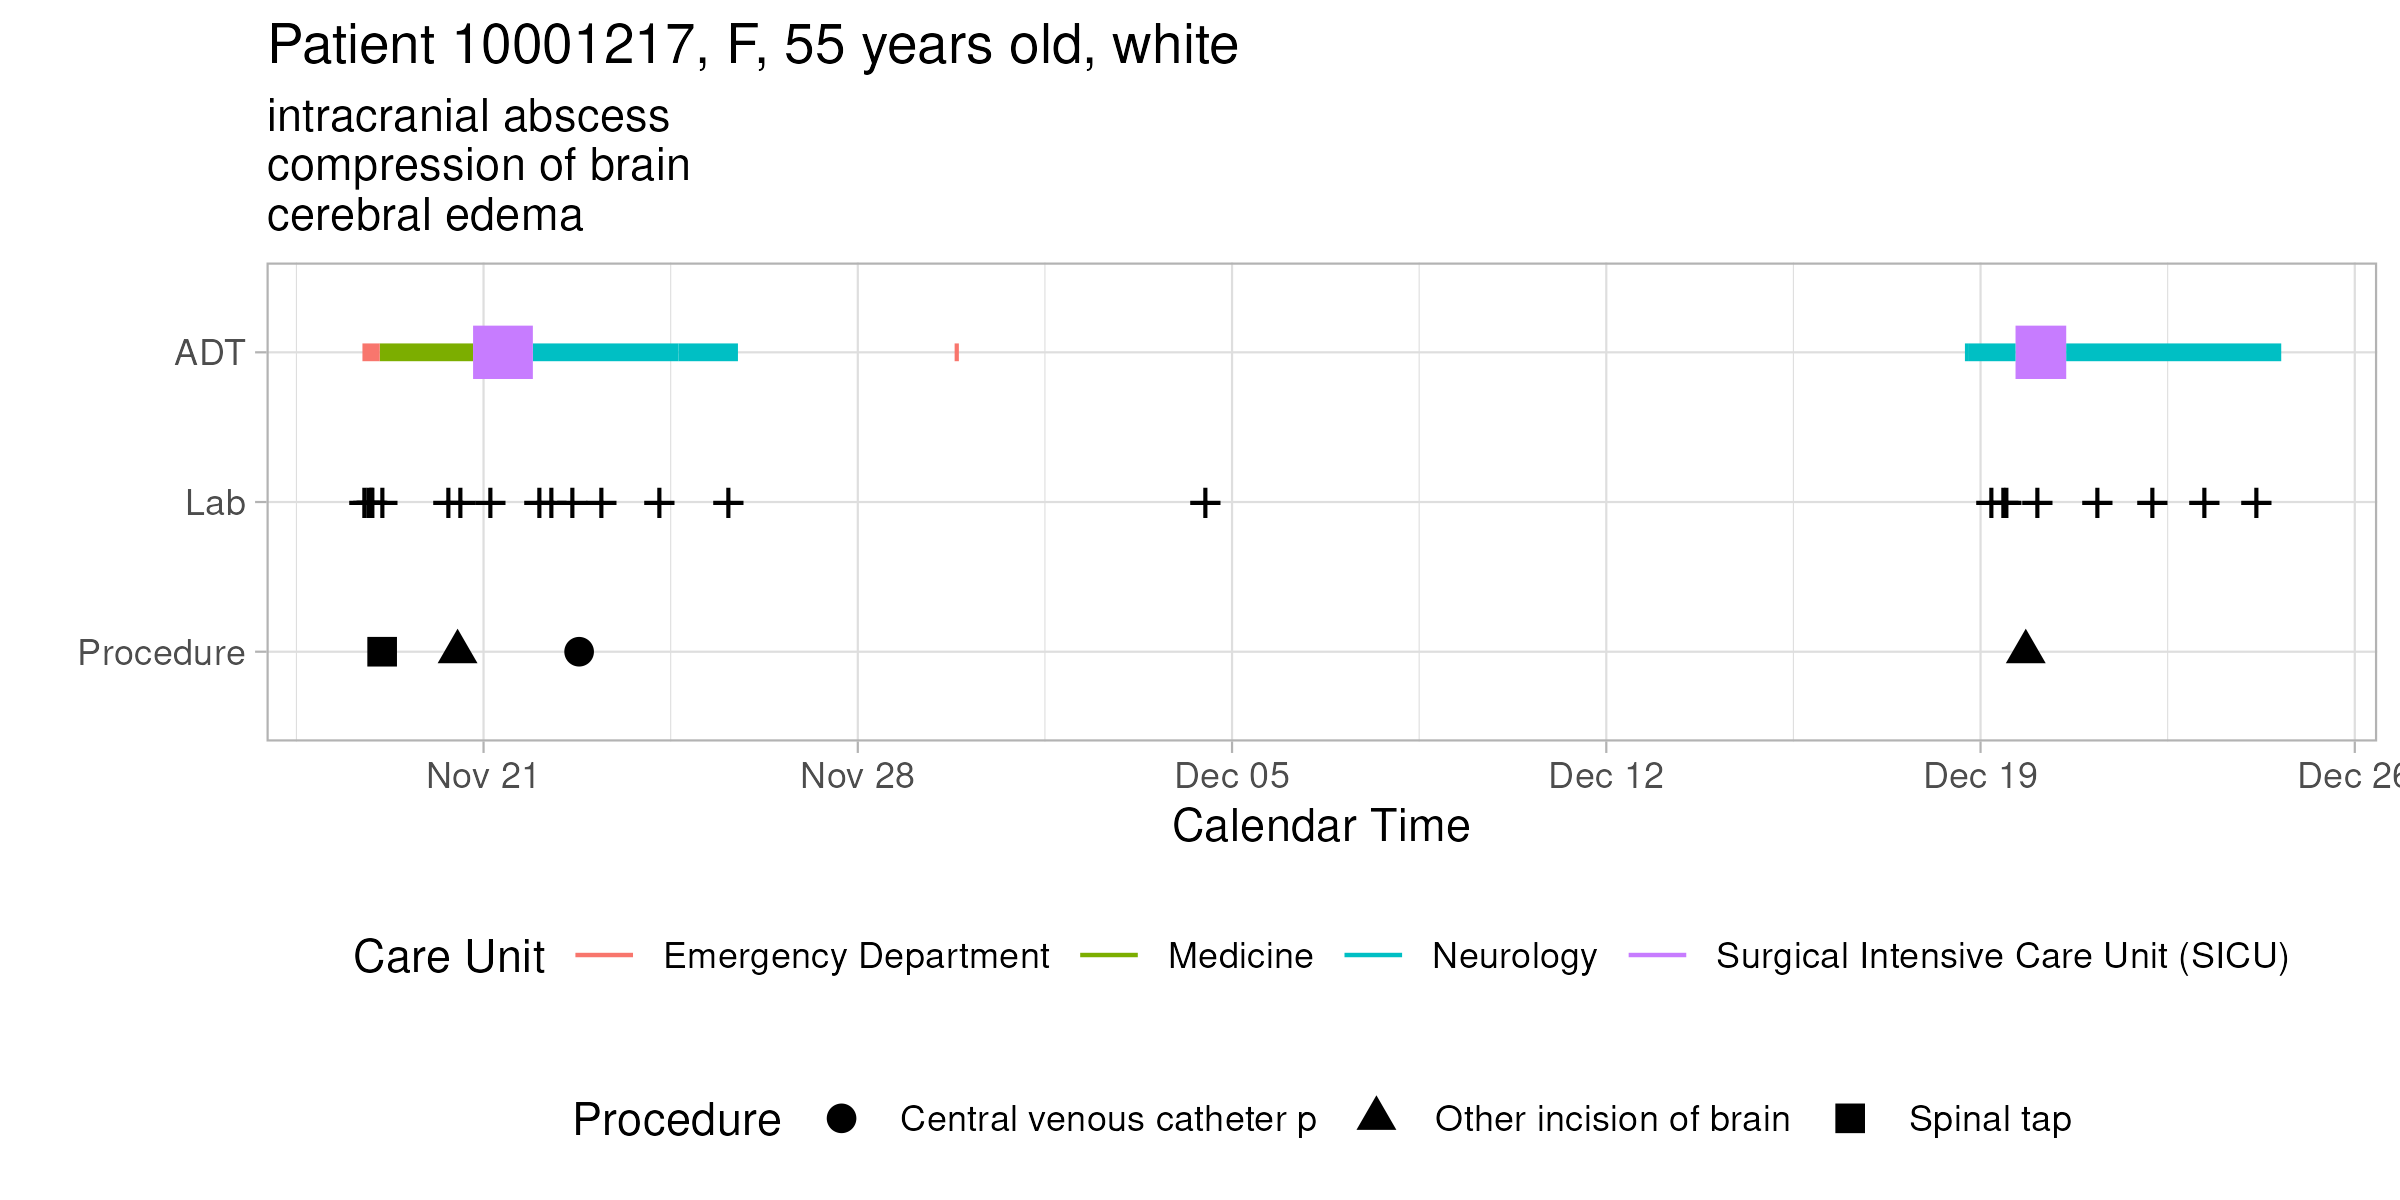
\includegraphics{images/10001217_adt.png} Do a similar visualization for
the patient with \texttt{subject\_id} 10063848 using ggplot.

Hint: We need to pull information from data files
\texttt{patients.csv.gz}, \texttt{admissions.csv.gz},
\texttt{transfers.csv.gz}, \texttt{labevents.csv.gz},
\texttt{procedures\_icd.csv.gz}, \texttt{diagnoses\_icd.csv.gz},
\texttt{d\_icd\_procedures.csv.gz}, and
\texttt{d\_icd\_diagnoses.csv.gz}. For the big file
\texttt{labevents.csv.gz}, use the Parquet format you generated in
Homework 2. For reproducibility, make the Parquet folder
\texttt{labevents\_pq} available at the current working directory
\texttt{hw3}, for example, by a symbolic link. Make your code
reproducible.

\begin{center}\rule{0.5\linewidth}{0.5pt}\end{center}

Solution:

\begin{Shaded}
\begin{Highlighting}[]
\CommentTok{\# Load datasets as tbles}
\NormalTok{patients }\OtherTok{\textless{}{-}} \FunctionTok{read\_csv}\NormalTok{(}\StringTok{"\textasciitilde{}/mimic/hosp/patients.csv.gz"}\NormalTok{)}
\end{Highlighting}
\end{Shaded}

\begin{verbatim}
Rows: 364627 Columns: 6
-- Column specification --------------------------------------------------------
Delimiter: ","
chr  (2): gender, anchor_year_group
dbl  (3): subject_id, anchor_age, anchor_year
date (1): dod

i Use `spec()` to retrieve the full column specification for this data.
i Specify the column types or set `show_col_types = FALSE` to quiet this message.
\end{verbatim}

\begin{Shaded}
\begin{Highlighting}[]
\NormalTok{admissions }\OtherTok{\textless{}{-}} \FunctionTok{read\_csv}\NormalTok{(}\StringTok{"\textasciitilde{}/mimic/hosp/admissions.csv.gz"}\NormalTok{)}
\end{Highlighting}
\end{Shaded}

\begin{verbatim}
Rows: 546028 Columns: 16
-- Column specification --------------------------------------------------------
Delimiter: ","
chr  (8): admission_type, admit_provider_id, admission_location, discharge_l...
dbl  (3): subject_id, hadm_id, hospital_expire_flag
dttm (5): admittime, dischtime, deathtime, edregtime, edouttime

i Use `spec()` to retrieve the full column specification for this data.
i Specify the column types or set `show_col_types = FALSE` to quiet this message.
\end{verbatim}

\begin{Shaded}
\begin{Highlighting}[]
\NormalTok{transfers }\OtherTok{\textless{}{-}} \FunctionTok{read\_csv}\NormalTok{(}\StringTok{"\textasciitilde{}/mimic/hosp/transfers.csv.gz"}\NormalTok{)}
\end{Highlighting}
\end{Shaded}

\begin{verbatim}
Rows: 2413581 Columns: 7
-- Column specification --------------------------------------------------------
Delimiter: ","
chr  (2): eventtype, careunit
dbl  (3): subject_id, hadm_id, transfer_id
dttm (2): intime, outtime

i Use `spec()` to retrieve the full column specification for this data.
i Specify the column types or set `show_col_types = FALSE` to quiet this message.
\end{verbatim}

\begin{Shaded}
\begin{Highlighting}[]
\NormalTok{procedures }\OtherTok{\textless{}{-}} \FunctionTok{read\_csv}\NormalTok{(}\StringTok{"\textasciitilde{}/mimic/hosp/procedures\_icd.csv.gz"}\NormalTok{)}
\end{Highlighting}
\end{Shaded}

\begin{verbatim}
Rows: 859655 Columns: 6
-- Column specification --------------------------------------------------------
Delimiter: ","
chr  (1): icd_code
dbl  (4): subject_id, hadm_id, seq_num, icd_version
date (1): chartdate

i Use `spec()` to retrieve the full column specification for this data.
i Specify the column types or set `show_col_types = FALSE` to quiet this message.
\end{verbatim}

\begin{Shaded}
\begin{Highlighting}[]
\NormalTok{diagnoses }\OtherTok{\textless{}{-}} \FunctionTok{read\_csv}\NormalTok{(}\StringTok{"\textasciitilde{}/mimic/hosp/diagnoses\_icd.csv.gz"}\NormalTok{)}
\end{Highlighting}
\end{Shaded}

\begin{verbatim}
Rows: 6364488 Columns: 5
-- Column specification --------------------------------------------------------
Delimiter: ","
chr (1): icd_code
dbl (4): subject_id, hadm_id, seq_num, icd_version

i Use `spec()` to retrieve the full column specification for this data.
i Specify the column types or set `show_col_types = FALSE` to quiet this message.
\end{verbatim}

\begin{Shaded}
\begin{Highlighting}[]
\CommentTok{\# Filter for patient 10063848}
\NormalTok{patient\_id }\OtherTok{\textless{}{-}} \DecValTok{10063848}
\NormalTok{patient\_data }\OtherTok{\textless{}{-}}\NormalTok{ patients }\SpecialCharTok{\%\textgreater{}\%} \FunctionTok{filter}\NormalTok{(subject\_id }\SpecialCharTok{==}\NormalTok{ patient\_id)}
\NormalTok{admissions\_data }\OtherTok{\textless{}{-}}\NormalTok{ admissions }\SpecialCharTok{\%\textgreater{}\%} \FunctionTok{filter}\NormalTok{(subject\_id }\SpecialCharTok{==}\NormalTok{ patient\_id)}
\NormalTok{transfers\_data }\OtherTok{\textless{}{-}}\NormalTok{ transfers }\SpecialCharTok{\%\textgreater{}\%} \FunctionTok{filter}\NormalTok{(subject\_id }\SpecialCharTok{==}\NormalTok{ patient\_id)}
\NormalTok{procedures\_data }\OtherTok{\textless{}{-}}\NormalTok{ procedures }\SpecialCharTok{\%\textgreater{}\%} \FunctionTok{filter}\NormalTok{(subject\_id }\SpecialCharTok{==}\NormalTok{ patient\_id)}
\NormalTok{diagnoses\_data }\OtherTok{\textless{}{-}}\NormalTok{ diagnoses }\SpecialCharTok{\%\textgreater{}\%} \FunctionTok{filter}\NormalTok{(subject\_id }\SpecialCharTok{==}\NormalTok{ patient\_id)}
\NormalTok{d\_icd\_procedures }\OtherTok{\textless{}{-}} \FunctionTok{read\_csv}\NormalTok{(}\StringTok{"\textasciitilde{}/mimic/hosp/d\_icd\_procedures.csv.gz"}\NormalTok{)}
\end{Highlighting}
\end{Shaded}

\begin{verbatim}
Rows: 86423 Columns: 3
-- Column specification --------------------------------------------------------
Delimiter: ","
chr (2): icd_code, long_title
dbl (1): icd_version

i Use `spec()` to retrieve the full column specification for this data.
i Specify the column types or set `show_col_types = FALSE` to quiet this message.
\end{verbatim}

\begin{Shaded}
\begin{Highlighting}[]
\NormalTok{d\_icd\_diagnoses }\OtherTok{\textless{}{-}} \FunctionTok{read\_csv}\NormalTok{(}\StringTok{"\textasciitilde{}/mimic/hosp/d\_icd\_diagnoses.csv.gz"}\NormalTok{)}
\end{Highlighting}
\end{Shaded}

\begin{verbatim}
Rows: 112107 Columns: 3
-- Column specification --------------------------------------------------------
Delimiter: ","
chr (2): icd_code, long_title
dbl (1): icd_version

i Use `spec()` to retrieve the full column specification for this data.
i Specify the column types or set `show_col_types = FALSE` to quiet this message.
\end{verbatim}

\begin{Shaded}
\begin{Highlighting}[]
\FunctionTok{rm}\NormalTok{(patients,admissions,}
\NormalTok{   transfers,procedures,diagnoses,}
\NormalTok{   patient\_id)}
\end{Highlighting}
\end{Shaded}

\begin{Shaded}
\begin{Highlighting}[]
\CommentTok{\#Connect to DuckDB}
\NormalTok{con }\OtherTok{\textless{}{-}} \FunctionTok{dbConnect}\NormalTok{(duckdb}\SpecialCharTok{::}\FunctionTok{duckdb}\NormalTok{(), }\AttributeTok{dbdir =} \StringTok{":memory:"}\NormalTok{)}

\CommentTok{\#  Load \textasciigrave{}data\textasciigrave{} into DuckDB}
\FunctionTok{dbWriteTable}\NormalTok{(con, }\StringTok{"patients"}\NormalTok{, patient\_data, }\AttributeTok{overwrite =} \ConstantTok{TRUE}\NormalTok{)}
\FunctionTok{dbWriteTable}\NormalTok{(con, }\StringTok{"admissions"}\NormalTok{, admissions\_data, }\AttributeTok{overwrite =} \ConstantTok{TRUE}\NormalTok{)}
\FunctionTok{dbWriteTable}\NormalTok{(con, }\StringTok{"transfers"}\NormalTok{, transfers\_data, }\AttributeTok{overwrite =} \ConstantTok{TRUE}\NormalTok{)}
\FunctionTok{dbWriteTable}\NormalTok{(con, }\StringTok{"procedures"}\NormalTok{, procedures\_data, }\AttributeTok{overwrite =} \ConstantTok{TRUE}\NormalTok{)}
\FunctionTok{dbWriteTable}\NormalTok{(con, }\StringTok{"diagnoses"}\NormalTok{, diagnoses\_data, }\AttributeTok{overwrite =} \ConstantTok{TRUE}\NormalTok{)}
\FunctionTok{dbWriteTable}\NormalTok{(con, }\StringTok{"d\_icd\_procedures"}\NormalTok{, d\_icd\_procedures, }\AttributeTok{overwrite =} \ConstantTok{TRUE}\NormalTok{)}
\FunctionTok{dbWriteTable}\NormalTok{(con, }\StringTok{"d\_icd\_diagnoses"}\NormalTok{, d\_icd\_diagnoses, }\AttributeTok{overwrite =} \ConstantTok{TRUE}\NormalTok{)}
\end{Highlighting}
\end{Shaded}

\begin{Shaded}
\begin{Highlighting}[]
\CommentTok{\#  labevents}
\FunctionTok{dbExecute}\NormalTok{(con, }\StringTok{"CREATE TABLE Lab AS }
\StringTok{                SELECT subject\_id,hadm\_id,labevent\_id,}
\StringTok{                charttime,}
\StringTok{                FROM read\_parquet(}
\StringTok{    \textquotesingle{}\textasciitilde{}/biostat{-}203b{-}2025{-}winter/hw3/labevents\_parquet/\textquotesingle{} || }
\StringTok{    \textquotesingle{}part{-}0.parquet\textquotesingle{}}
\StringTok{  )}
\StringTok{                WHERE subject\_id = 10063848"}\NormalTok{)}
\end{Highlighting}
\end{Shaded}

\begin{verbatim}
[1] 1114
\end{verbatim}

\begin{Shaded}
\begin{Highlighting}[]
\CommentTok{\# ADT }
\FunctionTok{dbExecute}\NormalTok{(con, }\StringTok{"}
\StringTok{  CREATE TABLE ADT AS}
\StringTok{  SELECT}
\StringTok{    subject\_id,hadm\_id,}
\StringTok{    careunit,eventtype,}
\StringTok{    intime,outtime,}
\StringTok{  FROM transfers}
\StringTok{"}\NormalTok{)}
\end{Highlighting}
\end{Shaded}

\begin{verbatim}
[1] 15
\end{verbatim}

\begin{Shaded}
\begin{Highlighting}[]
\CommentTok{\# Procedures}
\FunctionTok{dbExecute}\NormalTok{(con, }\StringTok{"}
\StringTok{  CREATE TABLE Procedure AS}
\StringTok{  SELECT }
\StringTok{    p.subject\_id,p.hadm\_id,chartdate,  }
\StringTok{    dp.icd\_code,dp.icd\_version,dp.long\_title, }
\StringTok{  FROM procedures p}
\StringTok{  LEFT JOIN d\_icd\_procedures dp}
\StringTok{  ON p.icd\_code = dp.icd\_code and p.icd\_version = dp.icd\_version}
\StringTok{"}\NormalTok{)}
\end{Highlighting}
\end{Shaded}

\begin{verbatim}
[1] 6
\end{verbatim}

\begin{Shaded}
\begin{Highlighting}[]
\CommentTok{\#ADT history}
\FunctionTok{dbExecute}\NormalTok{(con, }\StringTok{"}
\StringTok{  CREATE TABLE ADT\_history AS}
\StringTok{  SELECT }
\StringTok{    a.subject\_id,a.hadm\_id,a.careunit,}
\StringTok{    a.eventtype,a.intime,a.outtime,}
\StringTok{    p.chartdate,p.long\_title, }
\StringTok{    p.chartdate,  }
\StringTok{  FROM ADT a}
\StringTok{  LEFT JOIN Procedure p}
\StringTok{  ON a.subject\_id = p.subject\_id and a.hadm\_id = p.hadm\_id}
\StringTok{"}\NormalTok{)}
\end{Highlighting}
\end{Shaded}

\begin{verbatim}
[1] 42
\end{verbatim}

\begin{Shaded}
\begin{Highlighting}[]
\CommentTok{\#patients info \& subtitle shows top 3 diagnoses.}
\FunctionTok{dbExecute}\NormalTok{(con, }\StringTok{"}
\StringTok{  CREATE TABLE title AS}
\StringTok{  SELECT }
\StringTok{    p.subject\_id,p.gender,p.anchor\_age,}
\StringTok{    d.icd\_code,d.icd\_version,}
\StringTok{    dd.long\_title, }
\StringTok{  FROM patients p}
\StringTok{  LEFT JOIN diagnoses d }
\StringTok{  on p.subject\_id = d.subject\_id }
\StringTok{  LEFT JOIN d\_icd\_diagnoses dd}
\StringTok{  ON d.icd\_code = dd.icd\_code and d.icd\_version = dd.icd\_version}
\StringTok{"}\NormalTok{)}
\end{Highlighting}
\end{Shaded}

\begin{verbatim}
[1] 34
\end{verbatim}

\begin{Shaded}
\begin{Highlighting}[]
\NormalTok{info }\OtherTok{\textless{}{-}} \FunctionTok{dbGetQuery}\NormalTok{(con, }\StringTok{"}
\StringTok{  SELECT t.subject\_id,t.gender,t.anchor\_age,a.race,}
\StringTok{  FROM title t}
\StringTok{  left join admissions a}
\StringTok{  on t.subject\_id = a.subject\_id}
\StringTok{  limit 1}
\StringTok{"}\NormalTok{)}
\end{Highlighting}
\end{Shaded}

\begin{Shaded}
\begin{Highlighting}[]
\NormalTok{top\_diagnoses }\OtherTok{\textless{}{-}} \FunctionTok{dbGetQuery}\NormalTok{(con, }\StringTok{"}
\StringTok{  SELECT dd.long\_title }
\StringTok{  FROM (}
\StringTok{    SELECT icd\_code }
\StringTok{    FROM diagnoses }
\StringTok{    LIMIT 3}
\StringTok{  ) AS t}
\StringTok{  LEFT JOIN d\_icd\_diagnoses dd}
\StringTok{    ON t.icd\_code = dd.icd\_code}
\StringTok{"}\NormalTok{)}

\NormalTok{top\_diagnoses\_vector }\OtherTok{\textless{}{-}}\NormalTok{ top\_diagnoses}\SpecialCharTok{$}\NormalTok{long\_title }

\FunctionTok{rm}\NormalTok{(top\_diagnoses)}
\end{Highlighting}
\end{Shaded}

\begin{Shaded}
\begin{Highlighting}[]
\CommentTok{\# Collect ADT Data}
\NormalTok{adt\_data }\OtherTok{\textless{}{-}} \FunctionTok{tbl}\NormalTok{(con, }\StringTok{"ADT\_history"}\NormalTok{) }\SpecialCharTok{\%\textgreater{}\%}
  \FunctionTok{collect}\NormalTok{() }\SpecialCharTok{\%\textgreater{}\%}
  \FunctionTok{mutate}\NormalTok{(}\AttributeTok{intime =} \FunctionTok{as.POSIXct}\NormalTok{(intime, }\AttributeTok{format=}\StringTok{"\%Y{-}\%m{-}\%d \%H:\%M:\%S"}\NormalTok{),}
         \AttributeTok{outtime =} \FunctionTok{as.POSIXct}\NormalTok{(outtime, }\AttributeTok{format=}\StringTok{"\%Y{-}\%m{-}\%d \%H:\%M:\%S"}\NormalTok{)) }\SpecialCharTok{\%\textgreater{}\%}
  \FunctionTok{filter}\NormalTok{(careunit }\SpecialCharTok{!=} \StringTok{"UNKNOWN"}\NormalTok{, outtime }\SpecialCharTok{\textgreater{}}\NormalTok{ intime)  }
\CommentTok{\# Remove unknown care units and ensure valid time intervals}

\CommentTok{\# Collect Procedure Data}
\NormalTok{procedure\_data }\OtherTok{\textless{}{-}} \FunctionTok{tbl}\NormalTok{(con, }\StringTok{"Procedure"}\NormalTok{) }\SpecialCharTok{\%\textgreater{}\%}
  \FunctionTok{collect}\NormalTok{() }\SpecialCharTok{\%\textgreater{}\%}
  \FunctionTok{mutate}\NormalTok{(}\AttributeTok{chartdate =} \FunctionTok{as.POSIXct}\NormalTok{(chartdate, }\AttributeTok{format=}\StringTok{"\%Y{-}\%m{-}\%d"}\NormalTok{))  }
\CommentTok{\# Convert chart date to POSIXct format}

\CommentTok{\# Collect Lab Data (Ensure One Cross Per Day)}
\NormalTok{lab\_data }\OtherTok{\textless{}{-}} \FunctionTok{tbl}\NormalTok{(con, }\StringTok{"Lab"}\NormalTok{) }\SpecialCharTok{\%\textgreater{}\%}
  \FunctionTok{collect}\NormalTok{() }\SpecialCharTok{\%\textgreater{}\%}
  \FunctionTok{mutate}\NormalTok{(}\AttributeTok{charttime =} \FunctionTok{as.POSIXct}\NormalTok{(charttime, }\AttributeTok{format=}\StringTok{"\%Y{-}\%m{-}\%d \%H:\%M:\%S"}\NormalTok{))  }
\CommentTok{\# Convert lab event timestamps to POSIXct format}

\CommentTok{\# Extract unique procedure names (long\_title)}
\NormalTok{unique\_shapes }\OtherTok{\textless{}{-}} \FunctionTok{unique}\NormalTok{(procedure\_data}\SpecialCharTok{$}\NormalTok{long\_title)}
\NormalTok{num\_shapes }\OtherTok{\textless{}{-}} \FunctionTok{length}\NormalTok{(unique\_shapes) }
\CommentTok{\# Count the number of unique procedure types}

\CommentTok{\# Preset shapes (circle, triangle, square)}
\NormalTok{base\_shapes }\OtherTok{\textless{}{-}} \FunctionTok{c}\NormalTok{(}\DecValTok{15}\NormalTok{,}\DecValTok{16}\NormalTok{,}\DecValTok{17}\NormalTok{)  }
\CommentTok{\# Default shapes for the first three procedures}

\CommentTok{\# Additional backup shapes (ggplot2 shape codes)}
\NormalTok{extra\_shapes }\OtherTok{\textless{}{-}} \FunctionTok{c}\NormalTok{(}\DecValTok{9}\NormalTok{,}\DecValTok{10}\NormalTok{,}\DecValTok{11}\NormalTok{,}\DecValTok{12}\NormalTok{,}\DecValTok{13}\NormalTok{,}\DecValTok{14}\NormalTok{)  }
\CommentTok{\# Extra shapes in case there are more procedure types}

\CommentTok{\# Determine the final set of shapes to use}
\ControlFlowTok{if}\NormalTok{ (num\_shapes }\SpecialCharTok{\textgreater{}} \FunctionTok{length}\NormalTok{(base\_shapes)) \{}
\NormalTok{  final\_shapes }\OtherTok{\textless{}{-}} \FunctionTok{c}\NormalTok{(base\_shapes, }
\NormalTok{                    extra\_shapes[}\DecValTok{1}\SpecialCharTok{:}\NormalTok{(num\_shapes }\SpecialCharTok{{-}} \FunctionTok{length}\NormalTok{(base\_shapes))])  }
  \CommentTok{\# Use backup shapes if needed}
\NormalTok{\} }\ControlFlowTok{else}\NormalTok{ \{}
\NormalTok{  final\_shapes }\OtherTok{\textless{}{-}}\NormalTok{ base\_shapes[}\DecValTok{1}\SpecialCharTok{:}\NormalTok{num\_shapes]  }
  \CommentTok{\# Use only the default shapes if they are enough}
\NormalTok{\}}

\CommentTok{\# Map procedure names to their corresponding shapes}
\NormalTok{shape\_mapping }\OtherTok{\textless{}{-}} \FunctionTok{setNames}\NormalTok{(final\_shapes, unique\_shapes)}
\end{Highlighting}
\end{Shaded}

\begin{Shaded}
\begin{Highlighting}[]
\CommentTok{\# Create Final Plot}
\NormalTok{final\_plot }\OtherTok{\textless{}{-}} \FunctionTok{ggplot}\NormalTok{() }\SpecialCharTok{+}
  
  \CommentTok{\# Procedure Events}
  \FunctionTok{geom\_point}\NormalTok{(}\AttributeTok{data =}\NormalTok{ procedure\_data, }\FunctionTok{aes}\NormalTok{(}\AttributeTok{x =}\NormalTok{ chartdate, }
                                        \AttributeTok{y =} \StringTok{"Procedure"}\NormalTok{, }
                                        \AttributeTok{shape =}\NormalTok{ long\_title), }\AttributeTok{size =} \DecValTok{5}\NormalTok{) }\SpecialCharTok{+}
  
  \CommentTok{\# Lab Events (Cross Shape)}
  \FunctionTok{geom\_point}\NormalTok{(}\AttributeTok{data =}\NormalTok{ lab\_data, }\FunctionTok{aes}\NormalTok{(}\AttributeTok{x =}\NormalTok{ charttime, }\AttributeTok{y =} \StringTok{"Lab"}\NormalTok{), }
             \AttributeTok{shape =} \DecValTok{3}\NormalTok{, }\AttributeTok{size =} \DecValTok{4}\NormalTok{, }\AttributeTok{stroke =} \FloatTok{1.5}\NormalTok{) }\SpecialCharTok{+}
  
  \CommentTok{\# ADT timeline}
  \FunctionTok{geom\_segment}\NormalTok{(}\AttributeTok{data =}\NormalTok{ adt\_data, }\FunctionTok{aes}\NormalTok{(}\AttributeTok{x =}\NormalTok{ intime, }\AttributeTok{xend =}\NormalTok{ outtime, }
                                    \AttributeTok{y =} \StringTok{"ADT"}\NormalTok{, }\AttributeTok{yend =} \StringTok{"ADT"}\NormalTok{, }
                                    \AttributeTok{color =}\NormalTok{ careunit, }
                                    \AttributeTok{size =} \FunctionTok{ifelse}\NormalTok{(careunit }\SpecialCharTok{\%in\%} \FunctionTok{c}\NormalTok{(}\StringTok{"}
\StringTok{                                    Surgical Intensive Care Unit (SICU)"}\NormalTok{, }
                                    \StringTok{"Medical Intensive Care Unit (MICU)"}\NormalTok{), }
                                    \DecValTok{10}\NormalTok{, }\DecValTok{5}\NormalTok{))) }\SpecialCharTok{+}

  \CommentTok{\# Dynamic Shape Assignment}
  \FunctionTok{scale\_shape\_manual}\NormalTok{(}\AttributeTok{values =}\NormalTok{ shape\_mapping) }\SpecialCharTok{+}  
  \FunctionTok{scale\_size\_identity}\NormalTok{() }\SpecialCharTok{+}  
  \FunctionTok{scale\_x\_datetime}\NormalTok{(}\AttributeTok{date\_labels =} \StringTok{"\%b \%d"}\NormalTok{, }\AttributeTok{date\_breaks =} \StringTok{"1 week"}\NormalTok{) }\SpecialCharTok{+}  

  \CommentTok{\# Axis Labels and Themes}
  \FunctionTok{labs}\NormalTok{(}\AttributeTok{title =} \FunctionTok{paste}\NormalTok{(}\StringTok{"Patient"}\NormalTok{, info[}\DecValTok{1}\NormalTok{], }\StringTok{","}\NormalTok{, }
\NormalTok{                     info[}\DecValTok{2}\NormalTok{], }\StringTok{","}\NormalTok{, info[}\DecValTok{3}\NormalTok{], }\StringTok{"years old,"}\NormalTok{,}
                     \FunctionTok{tolower}\NormalTok{(info[}\DecValTok{4}\NormalTok{])),}
       \AttributeTok{subtitle =} \FunctionTok{paste}\NormalTok{(top\_diagnoses\_vector, }\AttributeTok{collapse =} \StringTok{"}\SpecialCharTok{\textbackslash{}n}\StringTok{"}\NormalTok{),}
       \AttributeTok{x =} \StringTok{"Calendar Time"}\NormalTok{,}
       \AttributeTok{y =} \StringTok{""}\NormalTok{,}
       \AttributeTok{color =} \StringTok{"Care Unit"}\NormalTok{,}
       \AttributeTok{shape =} \StringTok{"Procedure"}\NormalTok{) }\SpecialCharTok{+}
  
  \FunctionTok{theme\_minimal}\NormalTok{() }\SpecialCharTok{+}
  \FunctionTok{theme}\NormalTok{(}\AttributeTok{legend.position =} \StringTok{"bottom"}\NormalTok{,  }\CommentTok{\# Move legend to the bottom}
        \AttributeTok{axis.text.y =} \FunctionTok{element\_text}\NormalTok{(}\AttributeTok{size =} \DecValTok{10}\NormalTok{),  }
        \CommentTok{\# Ensure Y{-}axis labels are readable}
        \AttributeTok{axis.ticks.y =} \FunctionTok{element\_blank}\NormalTok{()) }\SpecialCharTok{+}
  \FunctionTok{guides}\NormalTok{(}\AttributeTok{color =} \FunctionTok{guide\_legend}\NormalTok{(}\AttributeTok{nrow =} \DecValTok{6}\NormalTok{), }\AttributeTok{shape =} \FunctionTok{guide\_legend}\NormalTok{(}\AttributeTok{nrow =} \DecValTok{5}\NormalTok{))  }
\end{Highlighting}
\end{Shaded}

\begin{verbatim}
Warning: Using `size` aesthetic for lines was deprecated in ggplot2 3.4.0.
i Please use `linewidth` instead.
\end{verbatim}

\begin{Shaded}
\begin{Highlighting}[]
\CommentTok{\# Split legend into multiple rows}

\CommentTok{\# Save and display the plot}
\FunctionTok{ggsave}\NormalTok{(}\StringTok{"ADT\_plot.png"}\NormalTok{, final\_plot, }\AttributeTok{width =} \DecValTok{15}\NormalTok{, }\AttributeTok{height =} \DecValTok{6}\NormalTok{, }\AttributeTok{dpi =} \DecValTok{300}\NormalTok{)}
\FunctionTok{print}\NormalTok{(final\_plot)}
\end{Highlighting}
\end{Shaded}

\begin{figure}[H]

{\centering 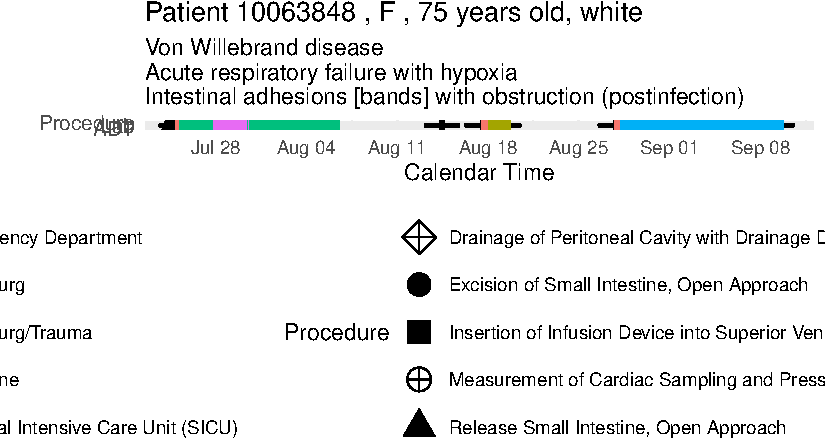
\includegraphics{hw3_files/figure-pdf/unnamed-chunk-6-1.pdf}

}

\end{figure}

\begin{Shaded}
\begin{Highlighting}[]
\FunctionTok{rm}\NormalTok{(top\_diagnoses\_vector)}
\end{Highlighting}
\end{Shaded}

\begin{Shaded}
\begin{Highlighting}[]
\FunctionTok{rm}\NormalTok{(admissions\_data,lab\_data,transfers\_data,}
\NormalTok{   procedure\_data,procedures\_data,d\_icd\_diagnoses,}
\NormalTok{   d\_icd\_procedures,patient\_data,adt\_data,diagnoses\_data)}

\FunctionTok{rm}\NormalTok{(final\_plot,shape\_mapping,unique\_shapes)}

\FunctionTok{rm}\NormalTok{(con,info)}
\end{Highlighting}
\end{Shaded}

\hypertarget{q1.2-icu-stays}{%
\subsubsection{Q1.2 ICU stays}\label{q1.2-icu-stays}}

ICU stays are a subset of ADT history. This figure shows the vitals of
the patient \texttt{10001217} during ICU stays. The x-axis is the
calendar time, and the y-axis is the value of the vital. The color of
the line represents the type of vital. The facet grid shows the
abbreviation of the vital and the stay ID.

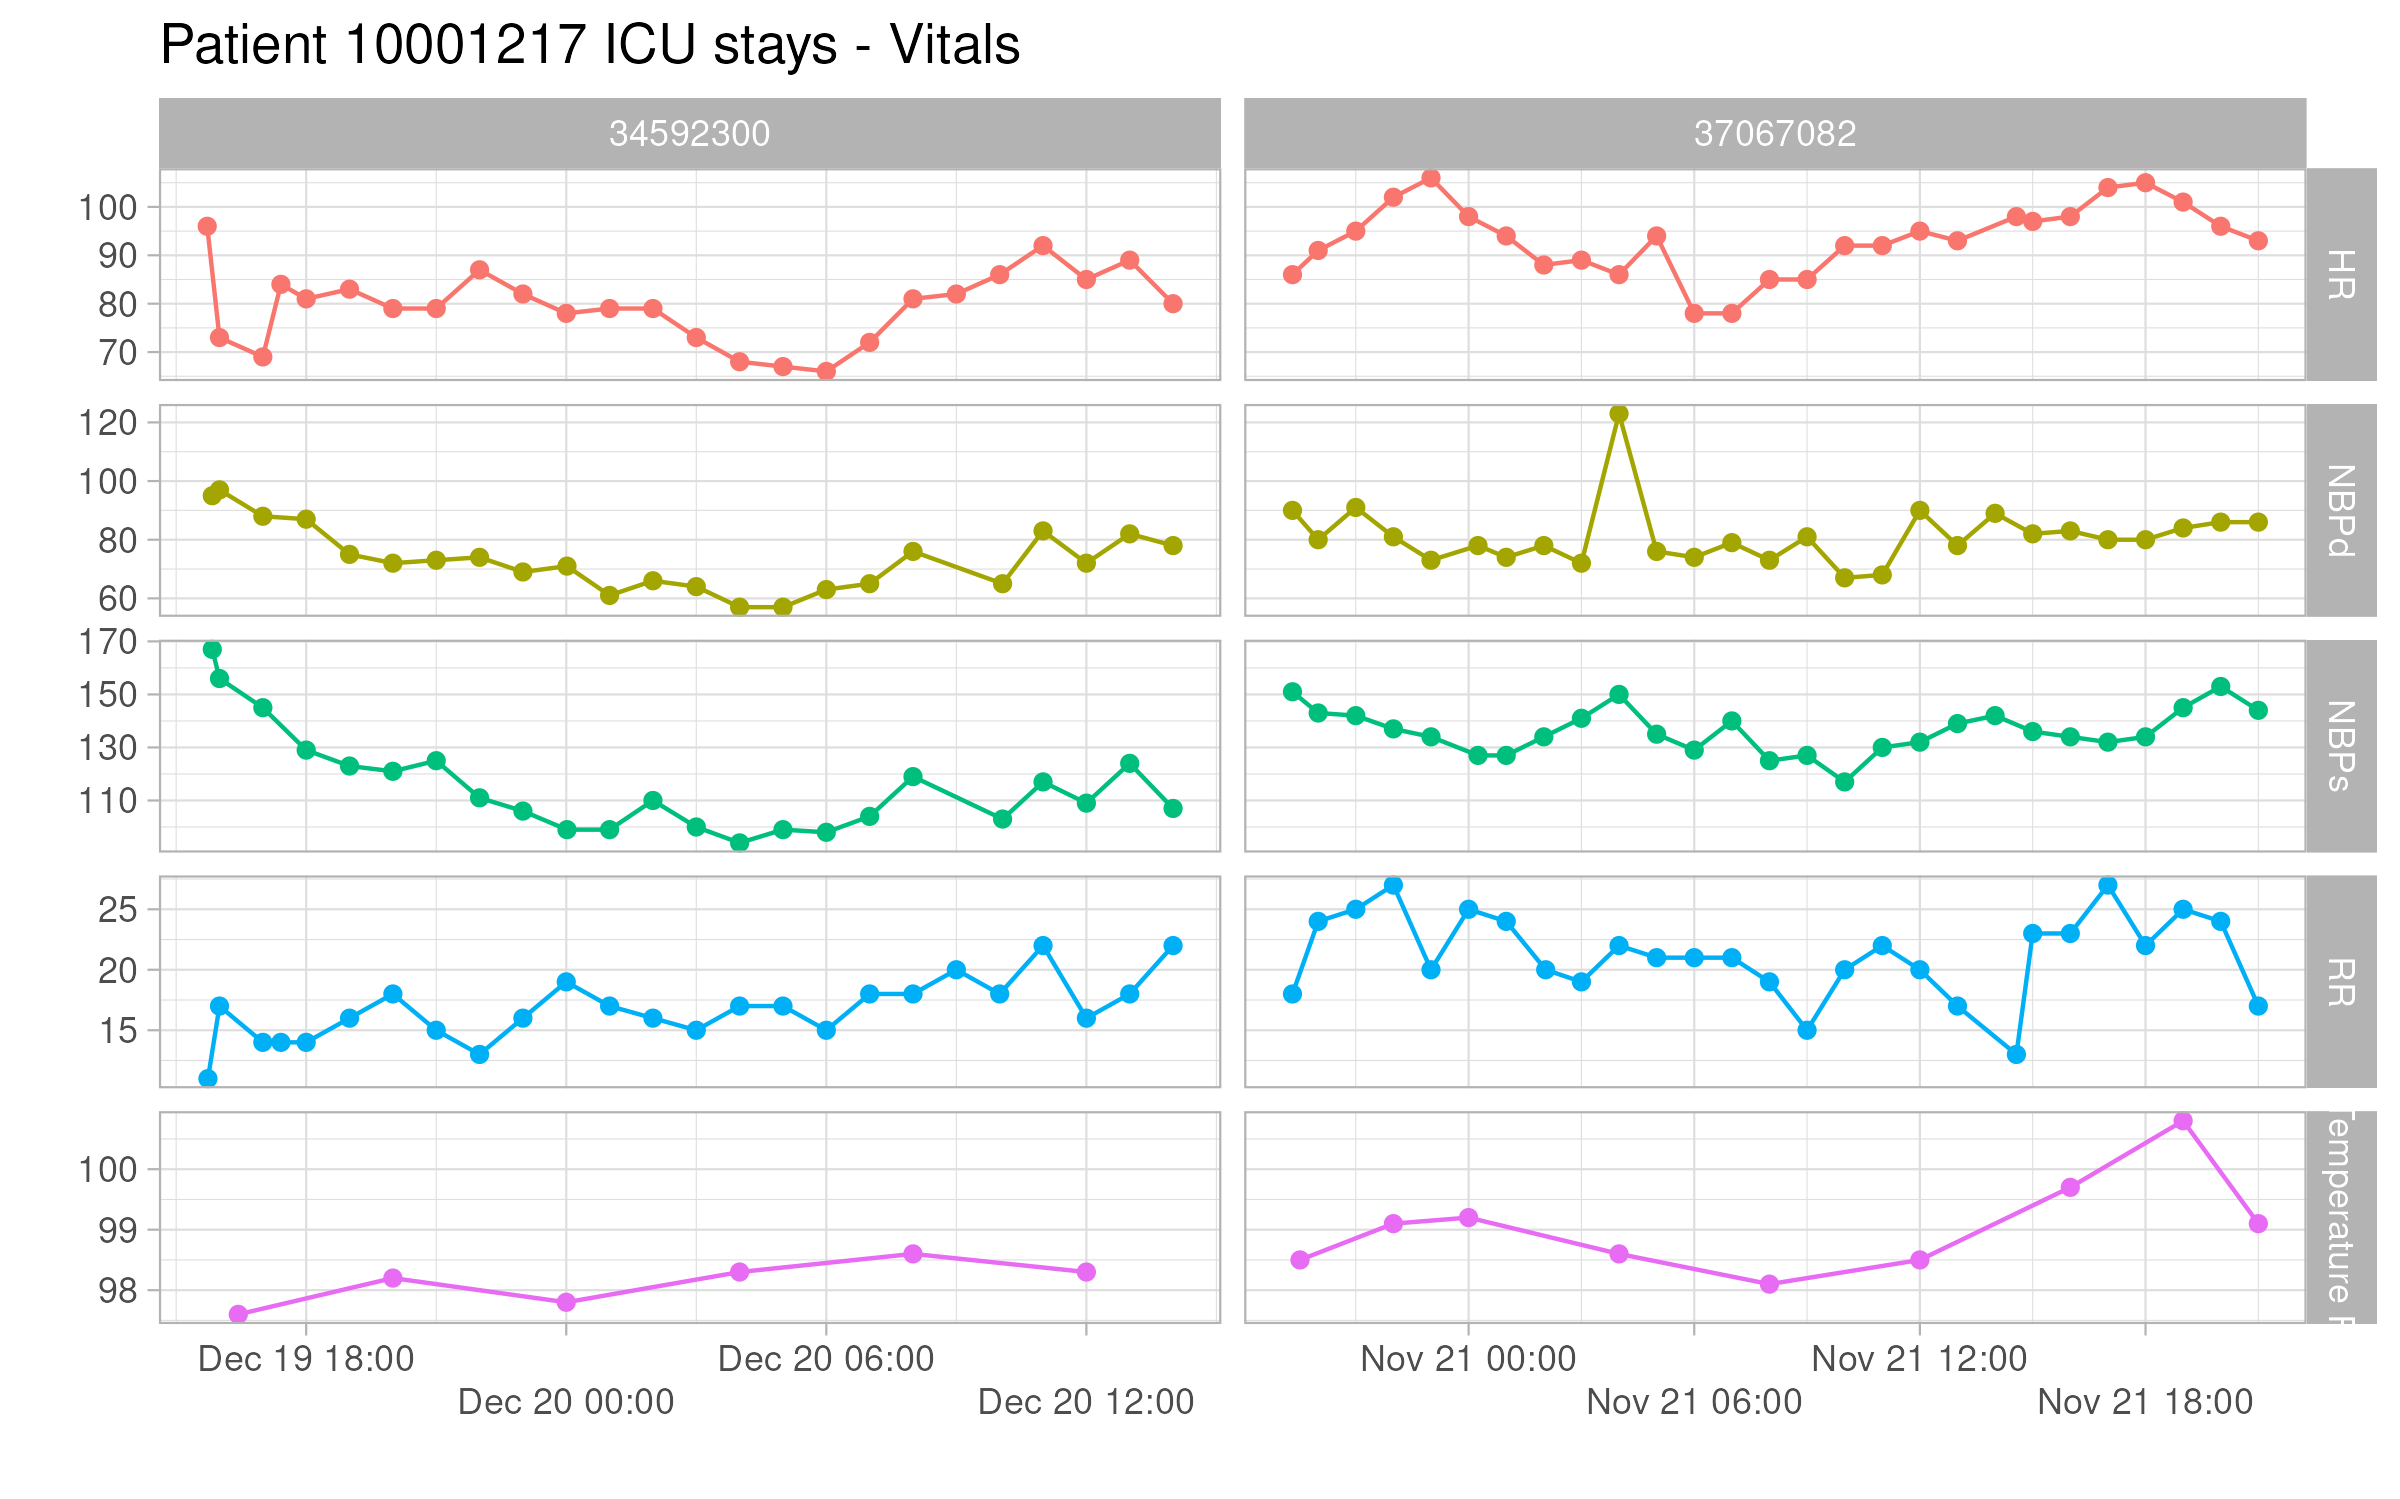
\includegraphics{images/10001217_icu.png}

Do a similar visualization for the patient \texttt{10063848}.

\begin{center}\rule{0.5\linewidth}{0.5pt}\end{center}

Solution:

\begin{Shaded}
\begin{Highlighting}[]
\NormalTok{patient\_id }\OtherTok{\textless{}{-}} \DecValTok{10063848}
\NormalTok{icustays }\OtherTok{\textless{}{-}} \FunctionTok{read\_csv}\NormalTok{(}\StringTok{"\textasciitilde{}/mimic/icu/icustays.csv.gz"}\NormalTok{)}
\end{Highlighting}
\end{Shaded}

\begin{verbatim}
Rows: 94458 Columns: 8
-- Column specification --------------------------------------------------------
Delimiter: ","
chr  (2): first_careunit, last_careunit
dbl  (4): subject_id, hadm_id, stay_id, los
dttm (2): intime, outtime

i Use `spec()` to retrieve the full column specification for this data.
i Specify the column types or set `show_col_types = FALSE` to quiet this message.
\end{verbatim}

\begin{Shaded}
\begin{Highlighting}[]
\NormalTok{patient\_data }\OtherTok{\textless{}{-}}\NormalTok{ icustays }\SpecialCharTok{\%\textgreater{}\%} \FunctionTok{filter}\NormalTok{(subject\_id }\SpecialCharTok{==}\NormalTok{ patient\_id)}
\end{Highlighting}
\end{Shaded}

\begin{Shaded}
\begin{Highlighting}[]
\CommentTok{\#Connect to DuckDB}
\NormalTok{con }\OtherTok{\textless{}{-}} \FunctionTok{dbConnect}\NormalTok{(duckdb}\SpecialCharTok{::}\FunctionTok{duckdb}\NormalTok{(), }\AttributeTok{dbdir =} \StringTok{":memory:"}\NormalTok{)}

\CommentTok{\#  Load \textasciigrave{}data\textasciigrave{} into DuckDB}
\FunctionTok{dbWriteTable}\NormalTok{(con, }\StringTok{"patients"}\NormalTok{, patient\_data, }\AttributeTok{overwrite =} \ConstantTok{TRUE}\NormalTok{)}
\FunctionTok{dbWriteTable}\NormalTok{(con, }\StringTok{"icustays"}\NormalTok{, icustays, }\AttributeTok{overwrite =} \ConstantTok{TRUE}\NormalTok{)}
\end{Highlighting}
\end{Shaded}

\begin{Shaded}
\begin{Highlighting}[]
\CommentTok{\# chartevents}
\FunctionTok{dbExecute}\NormalTok{(con, }\StringTok{"CREATE TABLE chartevents AS }
\StringTok{                SELECT subject\_id, itemid, charttime, valuenum }
\StringTok{                FROM read\_parquet(}
\StringTok{    \textquotesingle{}\textasciitilde{}/biostat{-}203b{-}2025{-}winter/hw3/chartevents\_parquet/\textquotesingle{} || }
\StringTok{    \textquotesingle{}part{-}0.parquet\textquotesingle{}}
\StringTok{  )}
\StringTok{                WHERE itemid IN (220045, 220179, 220180, 223761, 220210) and }
\StringTok{                subject\_id = 10063848"}\NormalTok{)}
\end{Highlighting}
\end{Shaded}

\begin{verbatim}
[1] 298
\end{verbatim}

\begin{Shaded}
\begin{Highlighting}[]
\CommentTok{\# stay }
\FunctionTok{dbExecute}\NormalTok{(con, }\StringTok{"}
\StringTok{  CREATE TABLE stay AS}
\StringTok{  SELECT subject\_id,stay\_id,intime,outtime}
\StringTok{  FROM icustays}
\StringTok{"}\NormalTok{)}
\end{Highlighting}
\end{Shaded}

\begin{verbatim}
[1] 94458
\end{verbatim}

\begin{Shaded}
\begin{Highlighting}[]
\CommentTok{\# vital}
\FunctionTok{dbExecute}\NormalTok{(con, }\StringTok{"}
\StringTok{  CREATE TABLE vital AS}
\StringTok{  SELECT c.subject\_id,c.itemid,}
\StringTok{  c.charttime,c.valuenum,}
\StringTok{  s.stay\_id,s.intime,s.outtime}
\StringTok{  FROM chartevents c}
\StringTok{  Left join stay s}
\StringTok{  on c.subject\_id = s.subject\_id}
\StringTok{"}\NormalTok{)}
\end{Highlighting}
\end{Shaded}

\begin{verbatim}
[1] 596
\end{verbatim}

\begin{Shaded}
\begin{Highlighting}[]
\CommentTok{\# Load data from DuckDB}
\NormalTok{vital\_data }\OtherTok{\textless{}{-}} \FunctionTok{dbGetQuery}\NormalTok{(con, }\StringTok{"}
\StringTok{  SELECT subject\_id, stay\_id, itemid, charttime,}
\StringTok{  valuenum, intime, outtime}
\StringTok{  FROM vital  }
\StringTok{  WHERE charttime BETWEEN intime AND outtime}
\StringTok{"}\NormalTok{)}

\FunctionTok{rm}\NormalTok{(icustays,patient\_data)}
\end{Highlighting}
\end{Shaded}

\begin{Shaded}
\begin{Highlighting}[]
\CommentTok{\# Convert time columns to POSIXct}
\NormalTok{vital\_data }\OtherTok{\textless{}{-}}\NormalTok{ vital\_data }\SpecialCharTok{\%\textgreater{}\%}
  \FunctionTok{mutate}\NormalTok{(}\AttributeTok{charttime =} \FunctionTok{as.POSIXct}\NormalTok{(charttime, }\AttributeTok{format=}\StringTok{"\%Y{-}\%m{-}\%d \%H:\%M:\%S"}\NormalTok{),}
         \AttributeTok{intime =} \FunctionTok{as.POSIXct}\NormalTok{(intime, }\AttributeTok{format=}\StringTok{"\%Y{-}\%m{-}\%d \%H:\%M:\%S"}\NormalTok{),}
         \AttributeTok{outtime =} \FunctionTok{as.POSIXct}\NormalTok{(outtime, }\AttributeTok{format=}\StringTok{"\%Y{-}\%m{-}\%d \%H:\%M:\%S"}\NormalTok{))}
  

\CommentTok{\# Define mapping for itemid to readable labels}
\NormalTok{itemid\_labels }\OtherTok{\textless{}{-}} \FunctionTok{c}\NormalTok{(}\StringTok{"220045"} \OtherTok{=} \StringTok{"HR"}\NormalTok{,}
                   \StringTok{"220180"} \OtherTok{=} \StringTok{"NBPd"}\NormalTok{,}
                   \StringTok{"220179"} \OtherTok{=} \StringTok{"NBPs"}\NormalTok{,}
                   \StringTok{"220210"} \OtherTok{=} \StringTok{"RR"}\NormalTok{,}
                   \StringTok{"223761"} \OtherTok{=} \StringTok{"Temperature (F)"}\NormalTok{)}

\CommentTok{\# Assign readable labels for itemid}
\NormalTok{vital\_data }\OtherTok{\textless{}{-}}\NormalTok{ vital\_data }\SpecialCharTok{\%\textgreater{}\%}
  \FunctionTok{mutate}\NormalTok{(}\AttributeTok{vital\_type =} \FunctionTok{factor}\NormalTok{(itemid\_labels[}\FunctionTok{as.character}\NormalTok{(itemid)], }
                             \AttributeTok{levels =}\NormalTok{ itemid\_labels))}

\NormalTok{vital\_colors }\OtherTok{\textless{}{-}} \FunctionTok{c}\NormalTok{(}\StringTok{"HR"} \OtherTok{=} \StringTok{"\#FD6349"}\NormalTok{, }
                  \StringTok{"NBPd"} \OtherTok{=} \StringTok{"goldenrod"}\NormalTok{, }
                  \StringTok{"NBPs"} \OtherTok{=} \StringTok{"green"}\NormalTok{, }
                  \StringTok{"Temperature (F)"} \OtherTok{=} \StringTok{"\#FF01FD"}\NormalTok{, }
                  \StringTok{"RR"} \OtherTok{=} \StringTok{"skyblue"}\NormalTok{)}
\end{Highlighting}
\end{Shaded}

\begin{Shaded}
\begin{Highlighting}[]
\CommentTok{\# Adjust each stay\_id\textquotesingle{}s x{-}axis to fit within its intime and outtime range}
\NormalTok{vital\_data\_filtered }\OtherTok{\textless{}{-}}\NormalTok{ vital\_data }\SpecialCharTok{\%\textgreater{}\%}
  \FunctionTok{group\_by}\NormalTok{(stay\_id) }\SpecialCharTok{\%\textgreater{}\%}
  \FunctionTok{ungroup}\NormalTok{()}

\NormalTok{vital\_plot }\OtherTok{\textless{}{-}} \FunctionTok{ggplot}\NormalTok{(vital\_data\_filtered, }\FunctionTok{aes}\NormalTok{(}\AttributeTok{x =}\NormalTok{ charttime, }
                                              \AttributeTok{y =}\NormalTok{ valuenum, }
                                              \AttributeTok{color =}\NormalTok{ vital\_type)) }\SpecialCharTok{+}
  \FunctionTok{geom\_point}\NormalTok{(}\AttributeTok{size =} \FloatTok{1.5}\NormalTok{) }\SpecialCharTok{+}
  \FunctionTok{geom\_line}\NormalTok{(}\FunctionTok{aes}\NormalTok{(}\AttributeTok{group =}\NormalTok{ vital\_type), }\AttributeTok{size =} \FloatTok{0.7}\NormalTok{) }\SpecialCharTok{+} 
  \FunctionTok{scale\_color\_manual}\NormalTok{(}\AttributeTok{values =}\NormalTok{ vital\_colors) }\SpecialCharTok{+}
  \FunctionTok{scale\_x\_datetime}\NormalTok{(}\AttributeTok{labels =} \FunctionTok{date\_format}\NormalTok{(}\StringTok{"\%b \%d \%H:\%M"}\NormalTok{), }\AttributeTok{breaks =} \StringTok{"6 hours"}\NormalTok{) }\SpecialCharTok{+} 
  \FunctionTok{facet\_grid}\NormalTok{(vital\_type }\SpecialCharTok{\textasciitilde{}}\NormalTok{ stay\_id, }\AttributeTok{scales =} \StringTok{"free\_y"}\NormalTok{, }\AttributeTok{switch =} \StringTok{"y"}\NormalTok{) }\SpecialCharTok{+}
  \FunctionTok{labs}\NormalTok{(}\AttributeTok{title =} \FunctionTok{paste}\NormalTok{(}\StringTok{"Patient"}\NormalTok{, }
                     \FunctionTok{unique}\NormalTok{(vital\_data}\SpecialCharTok{$}\NormalTok{subject\_id), }\StringTok{"ICU Stays {-} Vitals"}\NormalTok{),}
       \AttributeTok{x =} \StringTok{"ICU Admission (Intime) and Discharge (Outtime)"}\NormalTok{,}
       \AttributeTok{y =} \StringTok{"Value"}\NormalTok{) }\SpecialCharTok{+}  
  \FunctionTok{theme\_minimal}\NormalTok{() }\SpecialCharTok{+}
  \FunctionTok{theme}\NormalTok{(}\AttributeTok{axis.text.x =} \FunctionTok{element\_text}\NormalTok{(}\AttributeTok{angle =} \DecValTok{45}\NormalTok{, }\AttributeTok{hjust =} \DecValTok{1}\NormalTok{),}
        \AttributeTok{strip.placement =} \StringTok{"outside"}\NormalTok{,}
        \AttributeTok{strip.text.y.right =} \FunctionTok{element\_text}\NormalTok{(}\AttributeTok{size =} \DecValTok{12}\NormalTok{, }\AttributeTok{face =} \StringTok{"bold"}\NormalTok{),}
        \AttributeTok{legend.position =} \StringTok{"none"}\NormalTok{) }

\FunctionTok{ggsave}\NormalTok{(}\StringTok{"icu\_vitals.png"}\NormalTok{, vital\_plot, }\AttributeTok{width =} \DecValTok{12}\NormalTok{, }\AttributeTok{height =} \DecValTok{6}\NormalTok{, }\AttributeTok{dpi =} \DecValTok{300}\NormalTok{)}
\FunctionTok{print}\NormalTok{(vital\_plot)}
\end{Highlighting}
\end{Shaded}

\begin{figure}[H]

{\centering 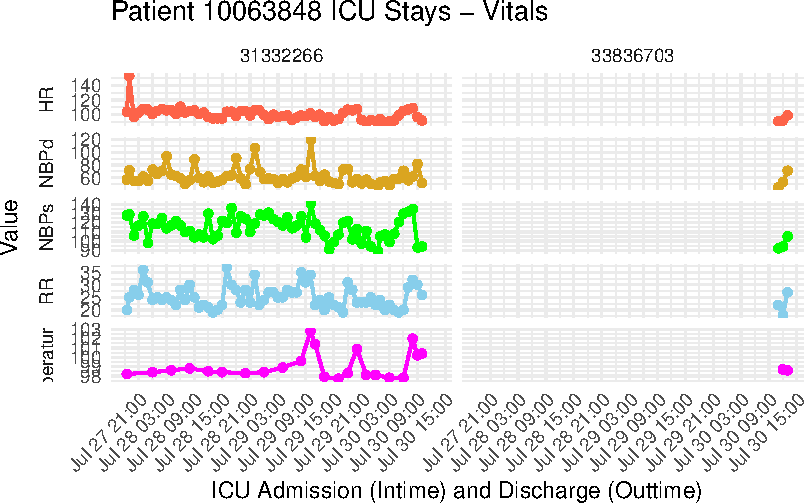
\includegraphics{hw3_files/figure-pdf/unnamed-chunk-15-1.pdf}

}

\end{figure}

\begin{Shaded}
\begin{Highlighting}[]
\FunctionTok{rm}\NormalTok{(vital\_data,vital\_data\_filtered,vital\_plot)}
\FunctionTok{rm}\NormalTok{(vital\_colors)}
\end{Highlighting}
\end{Shaded}

\hypertarget{q2.-icu-stays}{%
\subsection{Q2. ICU stays}\label{q2.-icu-stays}}

\texttt{icustays.csv.gz}
(\url{https://mimic.mit.edu/docs/iv/modules/icu/icustays/}) contains
data about Intensive Care Units (ICU) stays. The first 10 lines are

\begin{Shaded}
\begin{Highlighting}[]
\FunctionTok{zcat} \OperatorTok{\textless{}}\NormalTok{ \textasciitilde{}/mimic/icu/icustays.csv.gz }\KeywordTok{|} \FunctionTok{head}
\end{Highlighting}
\end{Shaded}

\hypertarget{q2.1-ingestion}{%
\subsubsection{Q2.1 Ingestion}\label{q2.1-ingestion}}

Import \texttt{icustays.csv.gz} as a tibble \texttt{icustays\_tble}.

\begin{center}\rule{0.5\linewidth}{0.5pt}\end{center}

Solution:

\begin{Shaded}
\begin{Highlighting}[]
\NormalTok{icustays\_tble }\OtherTok{\textless{}{-}} \FunctionTok{read\_csv}\NormalTok{(}\StringTok{"\textasciitilde{}/mimic/icu/icustays.csv.gz"}\NormalTok{)}
\end{Highlighting}
\end{Shaded}

\begin{verbatim}
Rows: 94458 Columns: 8
-- Column specification --------------------------------------------------------
Delimiter: ","
chr  (2): first_careunit, last_careunit
dbl  (4): subject_id, hadm_id, stay_id, los
dttm (2): intime, outtime

i Use `spec()` to retrieve the full column specification for this data.
i Specify the column types or set `show_col_types = FALSE` to quiet this message.
\end{verbatim}

\hypertarget{q2.2-summary-and-visualization}{%
\subsubsection{Q2.2 Summary and
visualization}\label{q2.2-summary-and-visualization}}

How many unique \texttt{subject\_id}? Can a \texttt{subject\_id} have
multiple ICU stays? Summarize the number of ICU stays per
\texttt{subject\_id} by graphs.

\begin{center}\rule{0.5\linewidth}{0.5pt}\end{center}

Solution:

\begin{Shaded}
\begin{Highlighting}[]
\CommentTok{\# Count unique subject\_id}
\NormalTok{num\_unique\_subjects }\OtherTok{\textless{}{-}}\NormalTok{ icustays\_tble}\SpecialCharTok{\%\textgreater{}\%} 
  \FunctionTok{distinct}\NormalTok{(subject\_id) }\SpecialCharTok{\%\textgreater{}\%} 
  \FunctionTok{nrow}\NormalTok{()}

\FunctionTok{print}\NormalTok{(}\FunctionTok{paste}\NormalTok{(}\StringTok{"Number of unique subjects:"}\NormalTok{, num\_unique\_subjects))}
\end{Highlighting}
\end{Shaded}

\begin{verbatim}
[1] "Number of unique subjects: 65366"
\end{verbatim}

\begin{Shaded}
\begin{Highlighting}[]
\FunctionTok{library}\NormalTok{(plotly)}
\end{Highlighting}
\end{Shaded}

\begin{verbatim}

Attaching package: 'plotly'
\end{verbatim}

\begin{verbatim}
The following object is masked from 'package:ggplot2':

    last_plot
\end{verbatim}

\begin{verbatim}
The following object is masked from 'package:arrow':

    schema
\end{verbatim}

\begin{verbatim}
The following object is masked from 'package:stats':

    filter
\end{verbatim}

\begin{verbatim}
The following object is masked from 'package:graphics':

    layout
\end{verbatim}

\begin{Shaded}
\begin{Highlighting}[]
\CommentTok{\# Count ICU stays per subject}
\NormalTok{icu\_stays\_per\_subject }\OtherTok{\textless{}{-}}\NormalTok{ icustays\_tble }\SpecialCharTok{\%\textgreater{}\%}
  \FunctionTok{group\_by}\NormalTok{(subject\_id) }\SpecialCharTok{\%\textgreater{}\%}
  \FunctionTok{summarise}\NormalTok{(}\AttributeTok{num\_stays =} \FunctionTok{n}\NormalTok{(), }\AttributeTok{.groups =} \StringTok{"drop"}\NormalTok{)}

\CommentTok{\# Create a histogram to visualize the distribution}
\NormalTok{p }\OtherTok{\textless{}{-}} \FunctionTok{ggplot}\NormalTok{(icu\_stays\_per\_subject, }\FunctionTok{aes}\NormalTok{(}\AttributeTok{x =}\NormalTok{ num\_stays)) }\SpecialCharTok{+}
  \FunctionTok{geom\_histogram}\NormalTok{(}\AttributeTok{binwidth =} \DecValTok{1}\NormalTok{, }\AttributeTok{fill =} \StringTok{"\#1B9E76"}\NormalTok{, }
                 \AttributeTok{color =} \StringTok{"black"}\NormalTok{, }\AttributeTok{alpha =} \FloatTok{0.7}\NormalTok{) }\SpecialCharTok{+}  
                  \CommentTok{\# Use histogram with bin width 1}
  \FunctionTok{scale\_x\_continuous}\NormalTok{(}\AttributeTok{limits =} \FunctionTok{c}\NormalTok{(}\DecValTok{0}\NormalTok{, }\DecValTok{30}\NormalTok{)) }\SpecialCharTok{+}  
  \CommentTok{\# Limit X{-}axis to focus on the majority of data}
  \FunctionTok{labs}\NormalTok{(}\AttributeTok{title =} \StringTok{"Distribution of ICU Stays per Subject"}\NormalTok{,}
       \AttributeTok{x =} \StringTok{"Number of ICU Stays"}\NormalTok{,}
       \AttributeTok{y =} \StringTok{"Count of Subjects"}\NormalTok{) }\SpecialCharTok{+}
  \FunctionTok{theme\_minimal}\NormalTok{()  }\CommentTok{\# Use a clean theme for better readability}

\FunctionTok{print}\NormalTok{(p)}
\end{Highlighting}
\end{Shaded}

\begin{verbatim}
Warning: Removed 4 rows containing non-finite outside the scale range
(`stat_bin()`).
\end{verbatim}

\begin{verbatim}
Warning: Removed 2 rows containing missing values or values outside the scale range
(`geom_bar()`).
\end{verbatim}

\begin{figure}[H]

{\centering 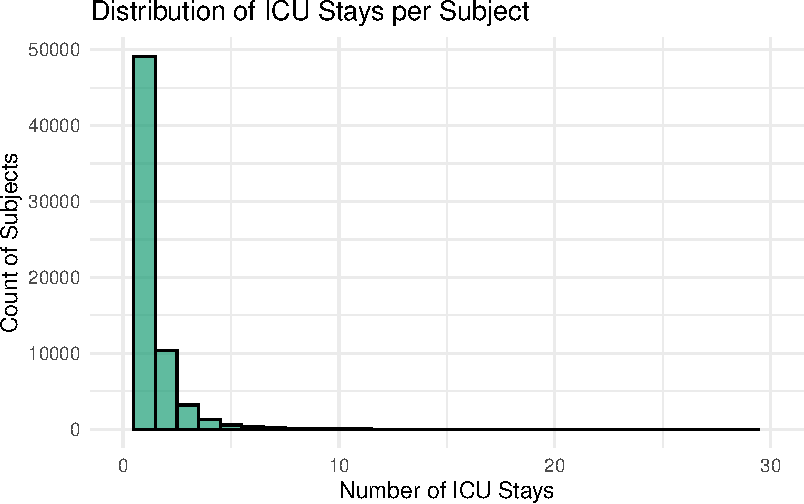
\includegraphics{hw3_files/figure-pdf/unnamed-chunk-20-1.pdf}

}

\end{figure}

\begin{Shaded}
\begin{Highlighting}[]
\CommentTok{\# Convert to an interactive plot}
\CommentTok{\#ggplotly(p)}

\FunctionTok{rm}\NormalTok{(icu\_stays\_per\_subject)}
\end{Highlighting}
\end{Shaded}

The histogram shows the distribution of ICU stays per subject (patient).
Most subjects have only one ICU stay, with a sharp drop-off as the
number of stays increases. The majority of patients (49,124 subjects)
had a single ICU stay, while a much smaller proportion experienced
multiple ICU stays. This suggests that repeated ICU admissions are
uncommon, but some patients do return multiple times, possibly due to
chronic conditions, post-surgical complications, or severe illnesses
requiring multiple admissions. The long tail of the distribution
indicates that a few patients had 10 or more ICU stays, though these
cases are rare.

\hypertarget{q3.-admissions-data}{%
\subsection{\texorpdfstring{Q3. \texttt{admissions}
data}{Q3. admissions data}}\label{q3.-admissions-data}}

Information of the patients admitted into hospital is available in
\texttt{admissions.csv.gz}. See
\url{https://mimic.mit.edu/docs/iv/modules/hosp/admissions/} for details
of each field in this file. The first 10 lines are

\begin{Shaded}
\begin{Highlighting}[]
\FunctionTok{zcat} \OperatorTok{\textless{}}\NormalTok{ \textasciitilde{}/mimic/hosp/admissions.csv.gz }\KeywordTok{|} \FunctionTok{head}
\end{Highlighting}
\end{Shaded}

\hypertarget{q3.1-ingestion}{%
\subsubsection{Q3.1 Ingestion}\label{q3.1-ingestion}}

Import \texttt{admissions.csv.gz} as a tibble \texttt{admissions\_tble}.

\begin{center}\rule{0.5\linewidth}{0.5pt}\end{center}

Solution:

\begin{Shaded}
\begin{Highlighting}[]
\NormalTok{admissions\_tble }\OtherTok{\textless{}{-}} \FunctionTok{read\_csv}\NormalTok{(}\StringTok{"\textasciitilde{}/mimic/hosp/admissions.csv.gz"}\NormalTok{)}
\end{Highlighting}
\end{Shaded}

\begin{verbatim}
Rows: 546028 Columns: 16
-- Column specification --------------------------------------------------------
Delimiter: ","
chr  (8): admission_type, admit_provider_id, admission_location, discharge_l...
dbl  (3): subject_id, hadm_id, hospital_expire_flag
dttm (5): admittime, dischtime, deathtime, edregtime, edouttime

i Use `spec()` to retrieve the full column specification for this data.
i Specify the column types or set `show_col_types = FALSE` to quiet this message.
\end{verbatim}

\hypertarget{q3.2-summary-and-visualization}{%
\subsubsection{Q3.2 Summary and
visualization}\label{q3.2-summary-and-visualization}}

Summarize the following information by graphics and explain any patterns
you see.

\begin{itemize}
\tightlist
\item
  number of admissions per patient\\
\item
  admission hour (anything unusual?)\\
\item
  admission minute (anything unusual?)\\
\item
  length of hospital stay (from admission to discharge) (anything
  unusual?)
\end{itemize}

According to the
\href{https://mimic.mit.edu/docs/iv/about/concepts/\#date-shifting}{MIMIC-IV
documentation},

\begin{quote}
All dates in the database have been shifted to protect patient
confidentiality. Dates will be internally consistent for the same
patient, but randomly distributed in the future. Dates of birth which
occur in the present time are not true dates of birth. Furthermore,
dates of birth which occur before the year 1900 occur if the patient is
older than 89. In these cases, the patient's age at their first
admission has been fixed to 300.
\end{quote}

\begin{center}\rule{0.5\linewidth}{0.5pt}\end{center}

Solution:

\begin{itemize}
\tightlist
\item
  \textbf{number of admissions per patient}
\end{itemize}

\begin{Shaded}
\begin{Highlighting}[]
\CommentTok{\# Compute the number of admissions per patient}
\NormalTok{admissions\_per\_patient }\OtherTok{\textless{}{-}}\NormalTok{ admissions\_tble }\SpecialCharTok{\%\textgreater{}\%}
  \FunctionTok{group\_by}\NormalTok{(subject\_id) }\SpecialCharTok{\%\textgreater{}\%}
  \FunctionTok{summarise}\NormalTok{(}\AttributeTok{num\_admissions =} \FunctionTok{n}\NormalTok{(), }\AttributeTok{.groups =} \StringTok{"drop"}\NormalTok{)}

\CommentTok{\# Create a histogram to visualize the distribution}
\NormalTok{p }\OtherTok{\textless{}{-}} \FunctionTok{ggplot}\NormalTok{(admissions\_per\_patient, }\FunctionTok{aes}\NormalTok{(}\AttributeTok{x =}\NormalTok{ num\_admissions)) }\SpecialCharTok{+}
  \FunctionTok{geom\_histogram}\NormalTok{(}\AttributeTok{binwidth =} \DecValTok{1}\NormalTok{, }\AttributeTok{fill =} \StringTok{"\#D81B60"}\NormalTok{, }
                 \AttributeTok{color =} \StringTok{"black"}\NormalTok{, }\AttributeTok{alpha =} \FloatTok{0.8}\NormalTok{) }\SpecialCharTok{+} 
                  \CommentTok{\# Use histogram instead of bar chart}
  \FunctionTok{scale\_x\_continuous}\NormalTok{(}\AttributeTok{limits =} \FunctionTok{c}\NormalTok{(}\DecValTok{0}\NormalTok{, }\DecValTok{30}\NormalTok{)) }\SpecialCharTok{+}  
  \CommentTok{\# Limit the X{-}axis to focus on the most relevant range}
  \FunctionTok{labs}\NormalTok{(}\AttributeTok{title =} \StringTok{"Number of Admissions per Patient"}\NormalTok{,}
       \AttributeTok{x =} \StringTok{"Admissions per Patient"}\NormalTok{,}
       \AttributeTok{y =} \StringTok{"Count of Patients"}\NormalTok{) }\SpecialCharTok{+}
  \FunctionTok{theme\_minimal}\NormalTok{()  }\CommentTok{\# Use a clean theme for better readability}

\FunctionTok{print}\NormalTok{(p)}
\end{Highlighting}
\end{Shaded}

\begin{verbatim}
Warning: Removed 504 rows containing non-finite outside the scale range
(`stat_bin()`).
\end{verbatim}

\begin{verbatim}
Warning: Removed 2 rows containing missing values or values outside the scale range
(`geom_bar()`).
\end{verbatim}

\begin{figure}[H]

{\centering 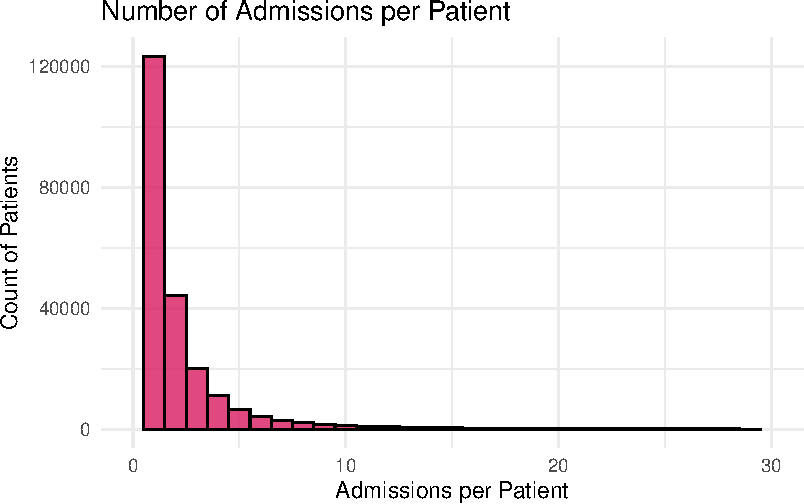
\includegraphics{hw3_files/figure-pdf/unnamed-chunk-23-1.pdf}

}

\end{figure}

\begin{Shaded}
\begin{Highlighting}[]
\CommentTok{\# Convert to an interactive plot}
\CommentTok{\#ggplotly(p)}

\FunctionTok{rm}\NormalTok{(admissions\_per\_patient)}
\end{Highlighting}
\end{Shaded}

Most patients have only one or very few admissions, while very few
patients have a large number of admissions. A small number of patients
have multiple hospitalizations, but the frequency drops quickly as the
number of admissions increases. Patients with 10+ admissions are very
rare. The distribution is heavily right-skewed, with very few patients
experiencing more than 5 hospital stays. This means that most patients
have a low number of admissions, and a small subset of patients has a
significantly higher number. Also, Most hospital patients are one-time
visitors, while a minority (likely with chronic illnesses or
complications) are readmitted multiple times.

\begin{itemize}
\tightlist
\item
  \textbf{admission hour (anything unusual?)}
\end{itemize}

\begin{Shaded}
\begin{Highlighting}[]
\CommentTok{\# Extract hour from admission time}
\NormalTok{admissions\_tble }\OtherTok{\textless{}{-}}\NormalTok{ admissions\_tble }\SpecialCharTok{\%\textgreater{}\%}
  \FunctionTok{mutate}\NormalTok{(}\AttributeTok{admission\_hour =} \FunctionTok{hour}\NormalTok{(admittime))}

\CommentTok{\# Create a histogram of admission hours}
\NormalTok{p\_hour }\OtherTok{\textless{}{-}} \FunctionTok{ggplot}\NormalTok{(admissions\_tble, }\FunctionTok{aes}\NormalTok{(}\AttributeTok{x =}\NormalTok{ admission\_hour)) }\SpecialCharTok{+}
  \FunctionTok{geom\_histogram}\NormalTok{(}\AttributeTok{binwidth =} \DecValTok{1}\NormalTok{, }\AttributeTok{fill =} \StringTok{"\#1E88E5"}\NormalTok{, }
                 \AttributeTok{color =} \StringTok{"black"}\NormalTok{, }\AttributeTok{alpha =} \FloatTok{0.8}\NormalTok{) }\SpecialCharTok{+}
  \FunctionTok{scale\_x\_continuous}\NormalTok{(}\AttributeTok{breaks =} \FunctionTok{seq}\NormalTok{(}\DecValTok{0}\NormalTok{, }\DecValTok{23}\NormalTok{, }\AttributeTok{by =} \DecValTok{1}\NormalTok{)) }\SpecialCharTok{+}
  \FunctionTok{labs}\NormalTok{(}\AttributeTok{title =} \StringTok{"Distribution of Admission Hours"}\NormalTok{,}
       \AttributeTok{x =} \StringTok{"Hour of Admission"}\NormalTok{,}
       \AttributeTok{y =} \StringTok{"Count of Admissions"}\NormalTok{) }\SpecialCharTok{+}
  \FunctionTok{theme\_minimal}\NormalTok{()}

\FunctionTok{print}\NormalTok{(p\_hour)}
\end{Highlighting}
\end{Shaded}

\begin{figure}[H]

{\centering 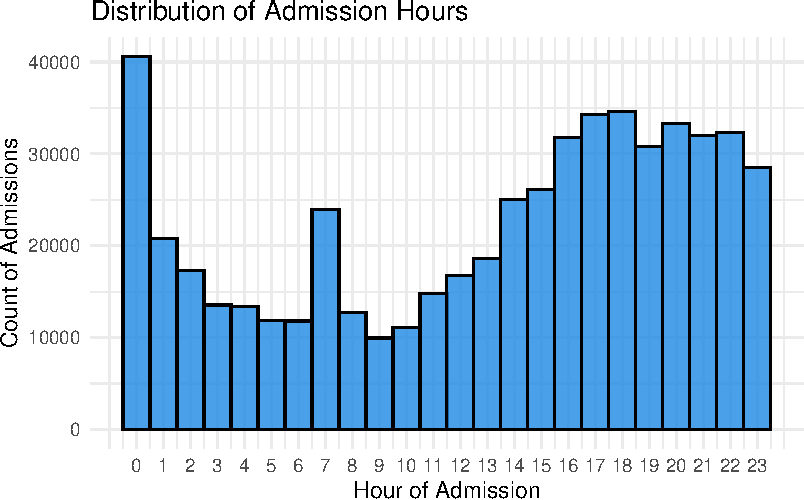
\includegraphics{hw3_files/figure-pdf/unnamed-chunk-24-1.pdf}

}

\end{figure}

\begin{Shaded}
\begin{Highlighting}[]
\CommentTok{\# Convert to interactive plot}
\CommentTok{\#ggplotly(p\_hour)}
\end{Highlighting}
\end{Shaded}

The distribution of admission hours shows notable patterns. There is a
sharp peak at midnight (00:00), suggesting that many admissions are
recorded at the start of the day, possibly due to administrative
rounding or batch processing of records. Another smaller peak is
observed around 07:00--08:00, which could be associated with morning
shift changes or scheduled hospital admissions. Admissions increase
steadily from late morning and peak between 16:00--19:00, likely
reflecting patient arrivals after daytime medical consultations and
emergency cases during evening hours. The pattern indicates a
combination of systemic recording practices, scheduled admissions, and
emergency patient arrivals.

\begin{itemize}
\tightlist
\item
  \textbf{admission minute (anything unusual?)}
\end{itemize}

\begin{Shaded}
\begin{Highlighting}[]
\CommentTok{\# Extract minute from admission time}
\NormalTok{admissions\_tble }\OtherTok{\textless{}{-}}\NormalTok{ admissions\_tble }\SpecialCharTok{\%\textgreater{}\%}
  \FunctionTok{mutate}\NormalTok{(}\AttributeTok{admission\_minute =} \FunctionTok{minute}\NormalTok{(admittime))}

\CommentTok{\# Create a histogram of admission minutes}
\NormalTok{p\_minute }\OtherTok{\textless{}{-}} \FunctionTok{ggplot}\NormalTok{(admissions\_tble, }\FunctionTok{aes}\NormalTok{(}\AttributeTok{x =}\NormalTok{ admission\_minute)) }\SpecialCharTok{+}
  \FunctionTok{geom\_histogram}\NormalTok{(}\AttributeTok{binwidth =} \DecValTok{1}\NormalTok{, }\AttributeTok{fill =} \StringTok{"\#FFC107"}\NormalTok{, }
                 \AttributeTok{color =} \StringTok{"black"}\NormalTok{, }\AttributeTok{alpha =} \FloatTok{0.8}\NormalTok{) }\SpecialCharTok{+}
  \FunctionTok{scale\_x\_continuous}\NormalTok{(}\AttributeTok{breaks =} \FunctionTok{seq}\NormalTok{(}\DecValTok{0}\NormalTok{, }\DecValTok{59}\NormalTok{, }\AttributeTok{by =} \DecValTok{5}\NormalTok{)) }\SpecialCharTok{+}
  \FunctionTok{labs}\NormalTok{(}\AttributeTok{title =} \StringTok{"Distribution of Admission Minutes"}\NormalTok{,}
       \AttributeTok{x =} \StringTok{"Minute of Admission"}\NormalTok{,}
       \AttributeTok{y =} \StringTok{"Count of Admissions"}\NormalTok{) }\SpecialCharTok{+}
  \FunctionTok{theme\_minimal}\NormalTok{()}

\FunctionTok{print}\NormalTok{(p\_minute)}
\end{Highlighting}
\end{Shaded}

\begin{figure}[H]

{\centering 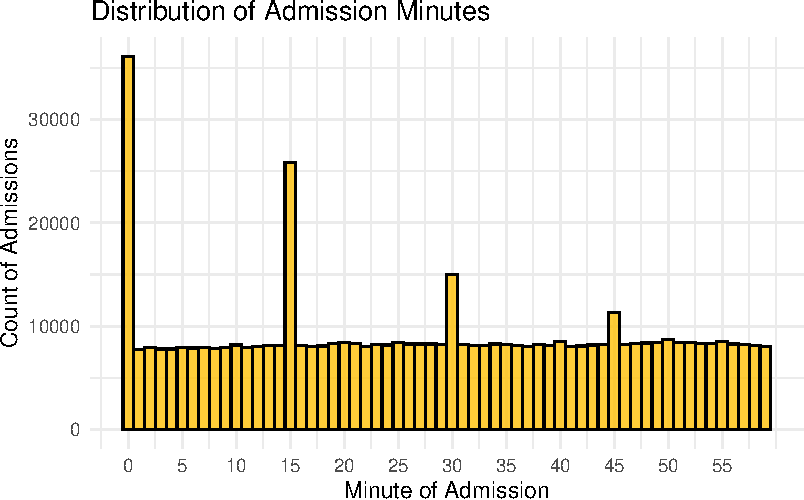
\includegraphics{hw3_files/figure-pdf/unnamed-chunk-25-1.pdf}

}

\end{figure}

\begin{Shaded}
\begin{Highlighting}[]
\CommentTok{\# Convert to interactive plot}
\CommentTok{\#ggplotly(p\_minute)}
\end{Highlighting}
\end{Shaded}

The distribution of admission minutes shows distinct spikes at 0, 15,
30, and 45 minutes, suggesting that admission times are often rounded to
quarter-hour intervals. This pattern likely arises due to manual data
entry practices, hospital system constraints, or administrative
processes that batch-record admissions. The relatively uniform
distribution in other minutes indicates that some admissions occur
naturally without rounding, but the spikes highlight a systemic bias in
how times are logged. This could impact time-based analyses and should
be accounted for in further data processing.

\begin{itemize}
\tightlist
\item
  \textbf{length of hospital stay (from admission to discharge)
  (anything unusual?)}
\end{itemize}

\begin{Shaded}
\begin{Highlighting}[]
\CommentTok{\# Calculate length of stay in days}
\NormalTok{admissions\_tble }\OtherTok{\textless{}{-}}\NormalTok{ admissions\_tble }\SpecialCharTok{\%\textgreater{}\%}
  \FunctionTok{mutate}\NormalTok{(}\AttributeTok{length\_of\_stay =} \FunctionTok{as.numeric}\NormalTok{(}\FunctionTok{difftime}\NormalTok{(dischtime, }
\NormalTok{                                              admittime, }\AttributeTok{units =} \StringTok{"days"}\NormalTok{)))}

\CommentTok{\# Create a histogram of hospital stay length}
\NormalTok{p\_los }\OtherTok{\textless{}{-}} \FunctionTok{ggplot}\NormalTok{(admissions\_tble, }\FunctionTok{aes}\NormalTok{(}\AttributeTok{x =}\NormalTok{ length\_of\_stay)) }\SpecialCharTok{+}
  \FunctionTok{geom\_histogram}\NormalTok{(}\AttributeTok{binwidth =} \DecValTok{1}\NormalTok{, }\AttributeTok{fill =} \StringTok{"\#4CAF50"}\NormalTok{, }
                 \AttributeTok{color =} \StringTok{"black"}\NormalTok{, }\AttributeTok{alpha =} \FloatTok{0.8}\NormalTok{) }\SpecialCharTok{+}
  \FunctionTok{scale\_x\_continuous}\NormalTok{(}\AttributeTok{limits =} \FunctionTok{c}\NormalTok{(}\DecValTok{0}\NormalTok{, }\DecValTok{50}\NormalTok{)) }\SpecialCharTok{+}  
  \CommentTok{\# Adjusted limit for visualization}
  \FunctionTok{labs}\NormalTok{(}\AttributeTok{title =} \StringTok{"Distribution of Hospital Stay Length"}\NormalTok{,}
       \AttributeTok{x =} \StringTok{"Length of Stay (Days)"}\NormalTok{,}
       \AttributeTok{y =} \StringTok{"Count of Admissions"}\NormalTok{) }\SpecialCharTok{+}
  \FunctionTok{theme\_minimal}\NormalTok{()}

\FunctionTok{print}\NormalTok{(p\_los)}
\end{Highlighting}
\end{Shaded}

\begin{verbatim}
Warning: Removed 2105 rows containing non-finite outside the scale range
(`stat_bin()`).
\end{verbatim}

\begin{verbatim}
Warning: Removed 2 rows containing missing values or values outside the scale range
(`geom_bar()`).
\end{verbatim}

\begin{figure}[H]

{\centering 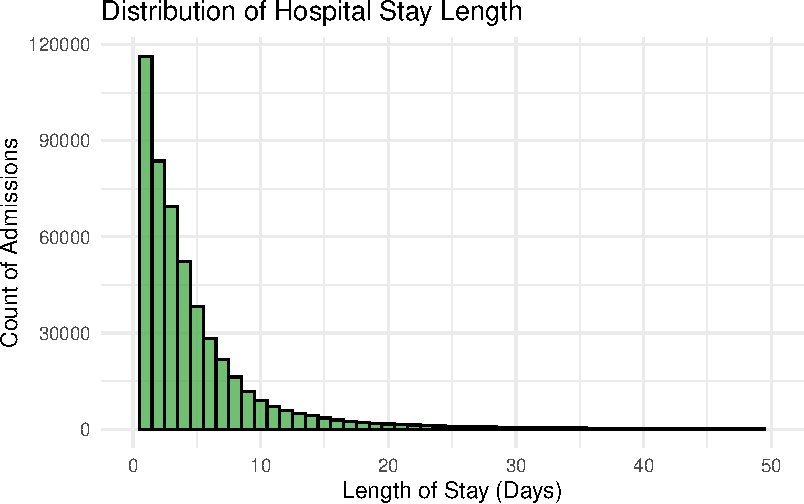
\includegraphics{hw3_files/figure-pdf/unnamed-chunk-26-1.pdf}

}

\end{figure}

\begin{Shaded}
\begin{Highlighting}[]
\CommentTok{\# Convert to interactive plot}
\CommentTok{\#ggplotly(p\_los)}
\end{Highlighting}
\end{Shaded}

The distribution of hospital stay length is right-skewed, with most
admissions having a short length of stay. The majority of patients are
discharged within a few days, with the highest count around 1--3 days,
suggesting that many hospital visits are for short-term treatments or
observations. As the length of stay increases, the number of admissions
decreases, indicating that extended hospitalizations are less common.
The presence of a long tail suggests that a small number of patients
require prolonged hospital care, possibly due to severe or chronic
conditions. This pattern is typical in hospital data, where most cases
are routine and resolved quickly, while complex cases require extended
stays.

\hypertarget{q4.-patients-data}{%
\subsection{\texorpdfstring{Q4. \texttt{patients}
data}{Q4. patients data}}\label{q4.-patients-data}}

Patient information is available in \texttt{patients.csv.gz}. See
\url{https://mimic.mit.edu/docs/iv/modules/hosp/patients/} for details
of each field in this file. The first 10 lines are

\begin{Shaded}
\begin{Highlighting}[]
\FunctionTok{zcat} \OperatorTok{\textless{}}\NormalTok{ \textasciitilde{}/mimic/hosp/patients.csv.gz }\KeywordTok{|} \FunctionTok{head}
\end{Highlighting}
\end{Shaded}

\hypertarget{q4.1-ingestion}{%
\subsubsection{Q4.1 Ingestion}\label{q4.1-ingestion}}

Import \texttt{patients.csv.gz}
(\url{https://mimic.mit.edu/docs/iv/modules/hosp/patients/}) as a tibble
\texttt{patients\_tble}.

\begin{center}\rule{0.5\linewidth}{0.5pt}\end{center}

Solution:

\begin{Shaded}
\begin{Highlighting}[]
\NormalTok{patients\_tble }\OtherTok{\textless{}{-}} \FunctionTok{read\_csv}\NormalTok{(}\StringTok{"\textasciitilde{}/mimic/hosp/patients.csv.gz"}\NormalTok{)}
\end{Highlighting}
\end{Shaded}

\begin{verbatim}
Rows: 364627 Columns: 6
-- Column specification --------------------------------------------------------
Delimiter: ","
chr  (2): gender, anchor_year_group
dbl  (3): subject_id, anchor_age, anchor_year
date (1): dod

i Use `spec()` to retrieve the full column specification for this data.
i Specify the column types or set `show_col_types = FALSE` to quiet this message.
\end{verbatim}

\hypertarget{q4.2-summary-and-visualization}{%
\subsubsection{Q4.2 Summary and
visualization}\label{q4.2-summary-and-visualization}}

Summarize variables \texttt{gender} and \texttt{anchor\_age} by
graphics, and explain any patterns you see.

\begin{center}\rule{0.5\linewidth}{0.5pt}\end{center}

Solution:

\begin{Shaded}
\begin{Highlighting}[]
\CommentTok{\# Count the number of patients by gender}
\NormalTok{gender\_dist }\OtherTok{\textless{}{-}}\NormalTok{ patients\_tble }\SpecialCharTok{\%\textgreater{}\%}
  \FunctionTok{count}\NormalTok{(gender)}

\CommentTok{\# Bar plot for gender distribution}
\NormalTok{p\_gender }\OtherTok{\textless{}{-}} \FunctionTok{ggplot}\NormalTok{(gender\_dist, }\FunctionTok{aes}\NormalTok{(}\AttributeTok{x =}\NormalTok{ gender, }\AttributeTok{y =}\NormalTok{ n, }\AttributeTok{fill =}\NormalTok{ gender)) }\SpecialCharTok{+}
  \FunctionTok{geom\_bar}\NormalTok{(}\AttributeTok{stat =} \StringTok{"identity"}\NormalTok{, }\AttributeTok{color =} \StringTok{"black"}\NormalTok{, }\AttributeTok{alpha =} \FloatTok{0.8}\NormalTok{) }\SpecialCharTok{+}
  \FunctionTok{labs}\NormalTok{(}\AttributeTok{title =} \StringTok{"Gender Distribution"}\NormalTok{,}
       \AttributeTok{x =} \StringTok{"Gender"}\NormalTok{,}
       \AttributeTok{y =} \StringTok{"Count of Patients"}\NormalTok{) }\SpecialCharTok{+}
  \FunctionTok{theme\_minimal}\NormalTok{()}


\FunctionTok{print}\NormalTok{(p\_gender)}
\end{Highlighting}
\end{Shaded}

\begin{figure}[H]

{\centering 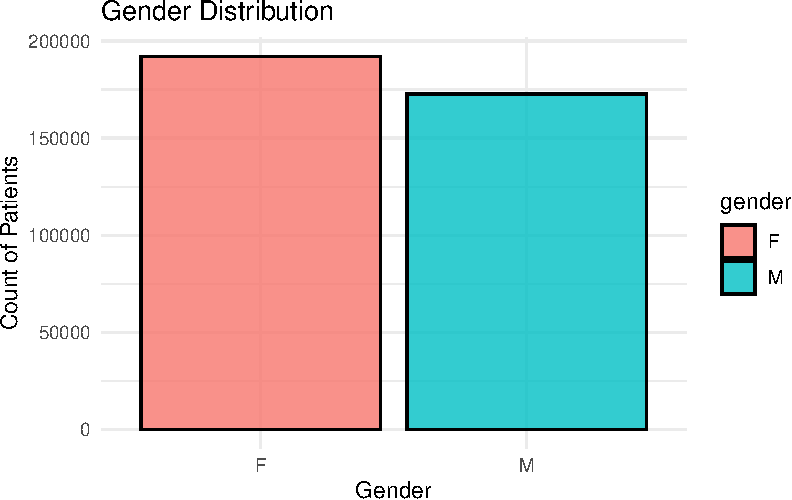
\includegraphics{hw3_files/figure-pdf/unnamed-chunk-29-1.pdf}

}

\end{figure}

\begin{Shaded}
\begin{Highlighting}[]
\CommentTok{\# Convert to interactive plot}
\CommentTok{\#ggplotly(p\_gender)}
\FunctionTok{rm}\NormalTok{(gender\_dist)}
\end{Highlighting}
\end{Shaded}

The bar chart indicates that there are more female (F) patients than
male (M) patients in the dataset. The difference is noticeable but not
extreme, suggesting a slight gender imbalance in hospital admissions.
This could be influenced by factors such as longer life expectancy in
females, higher healthcare utilization rates among women, or specific
hospital demographics.

\begin{Shaded}
\begin{Highlighting}[]
\CommentTok{\# Histogram of anchor\_age}
\NormalTok{p\_age }\OtherTok{\textless{}{-}} \FunctionTok{ggplot}\NormalTok{(patients\_tble, }\FunctionTok{aes}\NormalTok{(}\AttributeTok{x =}\NormalTok{ anchor\_age)) }\SpecialCharTok{+}
  \FunctionTok{geom\_histogram}\NormalTok{(}\AttributeTok{binwidth =} \DecValTok{5}\NormalTok{, }\AttributeTok{fill =} \StringTok{"\#1E88E5"}\NormalTok{, }
                 \AttributeTok{color =} \StringTok{"black"}\NormalTok{, }\AttributeTok{alpha =} \FloatTok{0.8}\NormalTok{) }\SpecialCharTok{+}
  \FunctionTok{labs}\NormalTok{(}\AttributeTok{title =} \StringTok{"Distribution of Anchor Age"}\NormalTok{,}
       \AttributeTok{x =} \StringTok{"Age (Years)"}\NormalTok{,}
       \AttributeTok{y =} \StringTok{"Count of Patients"}\NormalTok{) }\SpecialCharTok{+}
  \FunctionTok{theme\_minimal}\NormalTok{()}

\FunctionTok{print}\NormalTok{(p\_age)}
\end{Highlighting}
\end{Shaded}

\begin{figure}[H]

{\centering 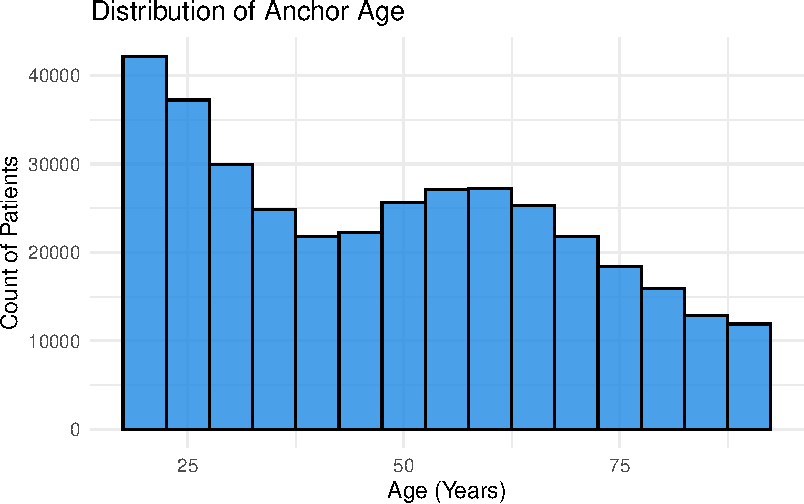
\includegraphics{hw3_files/figure-pdf/unnamed-chunk-30-1.pdf}

}

\end{figure}

\begin{Shaded}
\begin{Highlighting}[]
\CommentTok{\# Convert to interactive plot}
\CommentTok{\#ggplotly(p\_age)}
\end{Highlighting}
\end{Shaded}

The histogram of anchor\_age shows a bimodal distribution, with a large
concentration of patients in the 20--30 age range and another broader
peak between 50--70 years old. The younger peak could represent a large
number of maternity-related or younger adult admissions, while the older
peak likely reflects age-related chronic conditions and elderly care.
The drop-off after 80 years suggests a lower number of very elderly
patients, possibly due to lower life expectancy or selection bias in
hospital records.

\begin{Shaded}
\begin{Highlighting}[]
\FunctionTok{rm}\NormalTok{(p,p\_hour,p\_los,}
\NormalTok{   p\_minute,p\_gender,p\_age)}
\end{Highlighting}
\end{Shaded}

\hypertarget{q5.-lab-results}{%
\subsection{Q5. Lab results}\label{q5.-lab-results}}

\texttt{labevents.csv.gz}
(\url{https://mimic.mit.edu/docs/iv/modules/hosp/labevents/}) contains
all laboratory measurements for patients. The first 10 lines are

\begin{Shaded}
\begin{Highlighting}[]
\FunctionTok{zcat} \OperatorTok{\textless{}}\NormalTok{ \textasciitilde{}/mimic/hosp/labevents.csv.gz }\KeywordTok{|} \FunctionTok{head}
\end{Highlighting}
\end{Shaded}

\texttt{d\_labitems.csv.gz}
(\url{https://mimic.mit.edu/docs/iv/modules/hosp/d_labitems/}) is the
dictionary of lab measurements.

\begin{Shaded}
\begin{Highlighting}[]
\FunctionTok{zcat} \OperatorTok{\textless{}}\NormalTok{ \textasciitilde{}/mimic/hosp/d\_labitems.csv.gz }\KeywordTok{|} \FunctionTok{head}
\end{Highlighting}
\end{Shaded}

We are interested in the lab measurements of creatinine (50912),
potassium (50971), sodium (50983), chloride (50902), bicarbonate
(50882), hematocrit (51221), white blood cell count (51301), and glucose
(50931). Retrieve a subset of \texttt{labevents.csv.gz} that only
containing these items for the patients in \texttt{icustays\_tble}.
Further restrict to the last available measurement (by
\texttt{storetime}) before the ICU stay. The final
\texttt{labevents\_tble} should have one row per ICU stay and columns
for each lab measurement.

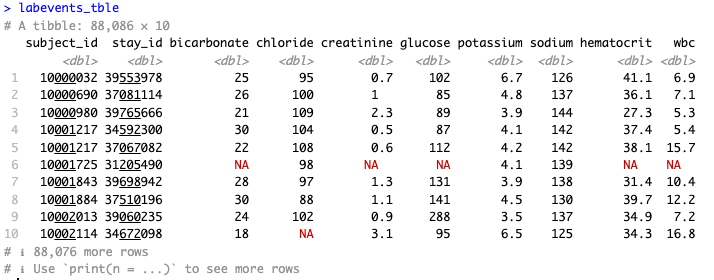
\includegraphics{images/labevents_tble.png}

Hint: Use the Parquet format you generated in Homework 2. For
reproducibility, make \texttt{labevents\_pq} folder available at the
current working directory \texttt{hw3}, for example, by a symbolic link.

\begin{center}\rule{0.5\linewidth}{0.5pt}\end{center}

Solution:

\begin{Shaded}
\begin{Highlighting}[]
\CommentTok{\# Connect to DuckDB}
\NormalTok{con }\OtherTok{\textless{}{-}} \FunctionTok{dbConnect}\NormalTok{(duckdb}\SpecialCharTok{::}\FunctionTok{duckdb}\NormalTok{(), }\AttributeTok{dbdir =} \StringTok{":memory:"}\NormalTok{)}

\CommentTok{\# Load and filter lab events directly in DuckDB}
\FunctionTok{dbExecute}\NormalTok{(con, }\StringTok{"CREATE TABLE filtered\_labevents AS }
\StringTok{                SELECT subject\_id, itemid, storetime, valuenum}
\StringTok{                FROM read\_parquet(}
\StringTok{    \textquotesingle{}\textasciitilde{}/biostat{-}203b{-}2025{-}winter/hw3/labevents\_parquet/\textquotesingle{} || }
\StringTok{    \textquotesingle{}part{-}0.parquet\textquotesingle{}}
\StringTok{  )}
\StringTok{                WHERE itemid IN (50912, 50971, 50983, 50902, }
\StringTok{          50882, 51221, 51301, 50931)"}\NormalTok{)}
\end{Highlighting}
\end{Shaded}

\begin{verbatim}
[1] 32679896
\end{verbatim}

\begin{Shaded}
\begin{Highlighting}[]
\CommentTok{\#  Load ICU stays dataset from CSV and store it in DuckDB}
\FunctionTok{dbExecute}\NormalTok{(con, }\StringTok{"CREATE TABLE icustays AS }
\StringTok{                SELECT subject\_id, stay\_id, intime, outtime }
\StringTok{                FROM read\_csv\_auto(\textquotesingle{}\textasciitilde{}/mimic/icu/icustays.csv.gz\textquotesingle{})"}\NormalTok{)}
\end{Highlighting}
\end{Shaded}

\begin{verbatim}
[1] 94458
\end{verbatim}

\begin{Shaded}
\begin{Highlighting}[]
\CommentTok{\# Join lab events with ICU stays and filter by time condition}
\FunctionTok{dbExecute}\NormalTok{(con, }\StringTok{"CREATE TABLE merged\_labevents AS }
\StringTok{                SELECT l.subject\_id, i.stay\_id, }
\StringTok{                l.itemid, l.storetime, l.valuenum}
\StringTok{                FROM filtered\_labevents l}
\StringTok{                INNER JOIN icustays i ON l.subject\_id = i.subject\_id}
\StringTok{                WHERE l.storetime \textless{} i.intime"}\NormalTok{)}
\end{Highlighting}
\end{Shaded}

\begin{verbatim}
[1] 20122551
\end{verbatim}

\begin{Shaded}
\begin{Highlighting}[]
\CommentTok{\# Select the most recent lab measurement per \textasciigrave{}itemid\textasciigrave{} before ICU admission}
\FunctionTok{dbExecute}\NormalTok{(con, }\StringTok{"CREATE TABLE latest\_labs AS }
\StringTok{                SELECT subject\_id, stay\_id, itemid, storetime, valuenum}
\StringTok{                FROM (}
\StringTok{                    SELECT *, ROW\_NUMBER() OVER (PARTITION BY }
\StringTok{                    subject\_id, stay\_id, itemid ORDER BY storetime DESC) AS rn}
\StringTok{                    FROM merged\_labevents}
\StringTok{                ) WHERE rn = 1"}\NormalTok{)}
\end{Highlighting}
\end{Shaded}

\begin{verbatim}
[1] 677237
\end{verbatim}

\begin{Shaded}
\begin{Highlighting}[]
\CommentTok{\# Pivot \textasciigrave{}itemid\textasciigrave{} to become separate columns}
\FunctionTok{dbExecute}\NormalTok{(con, }\StringTok{"CREATE TABLE labevents\_pivoted AS }
\StringTok{                SELECT subject\_id, stay\_id,}
\StringTok{                       MAX(CASE }
\StringTok{                       WHEN itemid = 50882 THEN valuenum END) AS bicarbonate,}
\StringTok{                       MAX(CASE }
\StringTok{                       WHEN itemid = 50902 THEN valuenum END) AS chloride,}
\StringTok{                       MAX(CASE }
\StringTok{                       WHEN itemid = 50912 THEN valuenum END) AS creatinine,}
\StringTok{                       MAX(CASE }
\StringTok{                       WHEN itemid = 50931 THEN valuenum END) AS glucose,}
\StringTok{                       MAX(CASE }
\StringTok{                       WHEN itemid = 50971 THEN valuenum END) AS potassium,}
\StringTok{                       MAX(CASE }
\StringTok{                       WHEN itemid = 50983 THEN valuenum END) AS sodium,}
\StringTok{                       MAX(CASE }
\StringTok{                       WHEN itemid = 51221 THEN valuenum END) AS hematocrit,}
\StringTok{                       MAX(CASE }
\StringTok{                       WHEN itemid = 51301 THEN valuenum END) AS wbc,}
\StringTok{                FROM latest\_labs}
\StringTok{                GROUP BY subject\_id, stay\_id"}\NormalTok{)}
\end{Highlighting}
\end{Shaded}

\begin{verbatim}
[1] 88086
\end{verbatim}

\begin{Shaded}
\begin{Highlighting}[]
\CommentTok{\# Fetch the final processed table into R}
\NormalTok{labevents\_tble }\OtherTok{\textless{}{-}} \FunctionTok{dbGetQuery}\NormalTok{(con, }\StringTok{"SELECT * FROM labevents\_pivoted"}\NormalTok{)}

\CommentTok{\# Arrange for better readability}
\NormalTok{labevents\_tble }\OtherTok{\textless{}{-}}\NormalTok{ labevents\_tble }\SpecialCharTok{\%\textgreater{}\%} \FunctionTok{arrange}\NormalTok{(subject\_id, stay\_id)}

\CommentTok{\# View final dataset}
\FunctionTok{options}\NormalTok{(}\AttributeTok{width =} \DecValTok{1000}\NormalTok{)}
\FunctionTok{print}\NormalTok{(}\FunctionTok{head}\NormalTok{(labevents\_tble, }\DecValTok{10}\NormalTok{))}
\end{Highlighting}
\end{Shaded}

\begin{verbatim}
   subject_id  stay_id bicarbonate chloride creatinine glucose potassium sodium hematocrit  wbc
1    10000032 39553978          25       95        0.7     102       6.7    126       41.1  6.9
2    10000690 37081114          26      100        1.0      85       4.8    137       36.1  7.1
3    10000980 39765666          21      109        2.3      89       3.9    144       27.3  5.3
4    10001217 34592300          30      104        0.5      87       4.1    142       37.4  5.4
5    10001217 37067082          22      108        0.6     112       4.2    142       38.1 15.7
6    10001725 31205490          NA       98         NA      NA       4.1    139         NA   NA
7    10001843 39698942          28       97        1.3     131       3.9    138       31.4 10.4
8    10001884 37510196          30       88        1.1     141       4.5    130       39.7 12.2
9    10002013 39060235          24      102        0.9     288       3.5    137       34.9  7.2
10   10002114 34672098          18       NA        3.1      95       6.5    125       34.3 16.8
\end{verbatim}

\begin{Shaded}
\begin{Highlighting}[]
\CommentTok{\# Disconnect from DuckDB}
\FunctionTok{dbDisconnect}\NormalTok{(con, }\AttributeTok{shutdown =} \ConstantTok{TRUE}\NormalTok{)}

\FunctionTok{rm}\NormalTok{(con)}
\FunctionTok{gc}\NormalTok{()}
\end{Highlighting}
\end{Shaded}

\begin{verbatim}
           used  (Mb) gc trigger  (Mb) max used  (Mb)
Ncells  1897047 101.4    3896008 208.1  3896008 208.1
Vcells 17232202 131.5   53504189 408.3 83584938 637.8
\end{verbatim}

\hypertarget{q6.-vitals-from-charted-events}{%
\subsection{Q6. Vitals from charted
events}\label{q6.-vitals-from-charted-events}}

\texttt{chartevents.csv.gz}
(\url{https://mimic.mit.edu/docs/iv/modules/icu/chartevents/}) contains
all the charted data available for a patient. During their ICU stay, the
primary repository of a patient's information is their electronic chart.
The \texttt{itemid} variable indicates a single measurement type in the
database. The \texttt{value} variable is the value measured for
\texttt{itemid}. The first 10 lines of \texttt{chartevents.csv.gz} are

\begin{Shaded}
\begin{Highlighting}[]
\FunctionTok{zcat} \OperatorTok{\textless{}}\NormalTok{ \textasciitilde{}/mimic/icu/chartevents.csv.gz }\KeywordTok{|} \FunctionTok{head}
\end{Highlighting}
\end{Shaded}

\texttt{d\_items.csv.gz}
(\url{https://mimic.mit.edu/docs/iv/modules/icu/d_items/}) is the
dictionary for the \texttt{itemid} in \texttt{chartevents.csv.gz}.

\begin{Shaded}
\begin{Highlighting}[]
\FunctionTok{zcat} \OperatorTok{\textless{}}\NormalTok{ \textasciitilde{}/mimic/icu/d\_items.csv.gz }\KeywordTok{|} \FunctionTok{head}
\end{Highlighting}
\end{Shaded}

We are interested in the vitals for ICU patients: heart rate (220045),
systolic non-invasive blood pressure (220179), diastolic non-invasive
blood pressure (220180), body temperature in Fahrenheit (223761), and
respiratory rate (220210). Retrieve a subset of
\texttt{chartevents.csv.gz} only containing these items for the patients
in \texttt{icustays\_tble}. Further restrict to the first vital
measurement within the ICU stay. The final \texttt{chartevents\_tble}
should have one row per ICU stay and columns for each vital measurement.

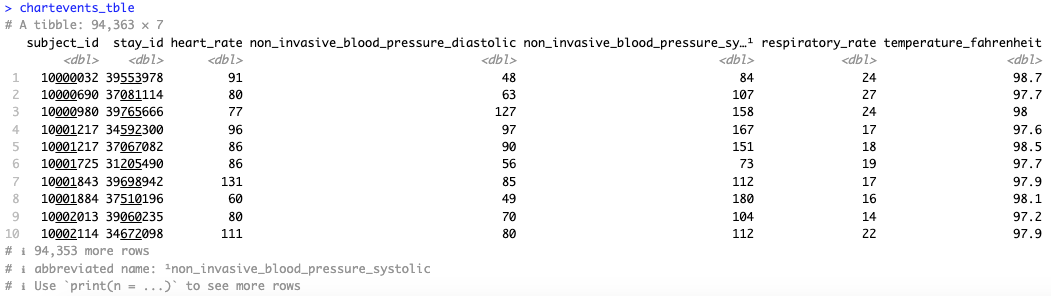
\includegraphics{images/clipboard-3810019433.png}Hint: Use the Parquet
format you generated in Homework 2. For reproducibility, make
\texttt{chartevents\_pq} folder available at the current working
directory, for example, by a symbolic link.

\begin{center}\rule{0.5\linewidth}{0.5pt}\end{center}

Solution:

\begin{Shaded}
\begin{Highlighting}[]
\CommentTok{\#Connect to DuckDB}
\NormalTok{con }\OtherTok{\textless{}{-}} \FunctionTok{dbConnect}\NormalTok{(duckdb}\SpecialCharTok{::}\FunctionTok{duckdb}\NormalTok{(), }\AttributeTok{dbdir =} \StringTok{":memory:"}\NormalTok{)}

\CommentTok{\# Load ICU stays dataset from CSV into DuckDB}
\NormalTok{duckdb\_table\_icustays }\OtherTok{\textless{}{-}} \FunctionTok{tbl}\NormalTok{(}
\NormalTok{  con, }\FunctionTok{sql}\NormalTok{(}\StringTok{"SELECT * FROM read\_csv\_auto(\textquotesingle{}\textasciitilde{}/mimic/icu/icustays.csv.gz\textquotesingle{})"}\NormalTok{)}
\NormalTok{  )}

\CommentTok{\# Query ICU stays dataset within DuckDB}
\NormalTok{result\_icustays }\OtherTok{\textless{}{-}}\NormalTok{ duckdb\_table\_icustays }\SpecialCharTok{\%\textgreater{}\%}
  \FunctionTok{select}\NormalTok{(subject\_id, stay\_id, intime,outtime) }\SpecialCharTok{\%\textgreater{}\%}  \CommentTok{\# Select necessary columns}
  \FunctionTok{collect}\NormalTok{()  }\CommentTok{\# Bring the filtered results into memory as a tibble}

\FunctionTok{dbDisconnect}\NormalTok{(con)}
\FunctionTok{gc}\NormalTok{()}
\end{Highlighting}
\end{Shaded}

\begin{verbatim}
           used  (Mb) gc trigger  (Mb) max used  (Mb)
Ncells  1921704 102.7    3896008 208.1  3896008 208.1
Vcells 17665157 134.8   53504189 408.3 83584938 637.8
\end{verbatim}

\begin{Shaded}
\begin{Highlighting}[]
\FunctionTok{rm}\NormalTok{(con,duckdb\_table\_icustays)}
\end{Highlighting}
\end{Shaded}

\begin{Shaded}
\begin{Highlighting}[]
\CommentTok{\# Connect to DuckDB}
\NormalTok{con }\OtherTok{\textless{}{-}} \FunctionTok{dbConnect}\NormalTok{(duckdb}\SpecialCharTok{::}\FunctionTok{duckdb}\NormalTok{(), }\AttributeTok{dbdir =} \StringTok{":memory:"}\NormalTok{) }

\CommentTok{\#  Load and filter only required \textasciigrave{}itemid\textasciigrave{} values (Reduce Memory Usage)}
\FunctionTok{dbExecute}\NormalTok{(con, }\StringTok{"CREATE TABLE chartevents\_duckdb AS }
\StringTok{                SELECT subject\_id, itemid, storetime, valuenum }
\StringTok{                FROM read\_parquet(}
\StringTok{    \textquotesingle{}\textasciitilde{}/biostat{-}203b{-}2025{-}winter/hw3/chartevents\_parquet/\textquotesingle{} || }
\StringTok{    \textquotesingle{}part{-}0.parquet\textquotesingle{}}
\StringTok{  )}
\StringTok{                WHERE itemid IN (220045, 220179, 220180, 223761, 220210)"}\NormalTok{)}
\end{Highlighting}
\end{Shaded}

\begin{verbatim}
[1] 30200193
\end{verbatim}

\begin{Shaded}
\begin{Highlighting}[]
\CommentTok{\#  Load \textasciigrave{}icustays\_tble\textasciigrave{} into DuckDB}
\FunctionTok{dbWriteTable}\NormalTok{(con, }\StringTok{"icustays"}\NormalTok{, result\_icustays, }\AttributeTok{overwrite =} \ConstantTok{TRUE}\NormalTok{)}
\end{Highlighting}
\end{Shaded}

\begin{Shaded}
\begin{Highlighting}[]
\CommentTok{\# Filter the measurements in between the icu time}
\FunctionTok{dbExecute}\NormalTok{(con, }\StringTok{"CREATE TABLE latest\_vitals\_raw AS }
\StringTok{                SELECT c.subject\_id, i.stay\_id, }
\StringTok{                c.itemid, c.storetime, c.valuenum}
\StringTok{                FROM chartevents\_duckdb c}
\StringTok{                INNER JOIN icustays i }
\StringTok{                ON c.subject\_id = i.subject\_id}
\StringTok{                WHERE c.storetime BETWEEN i.intime AND i.outtime"}\NormalTok{)}
\end{Highlighting}
\end{Shaded}

\begin{verbatim}
[1] 30129155
\end{verbatim}

\begin{Shaded}
\begin{Highlighting}[]
\FunctionTok{rm}\NormalTok{(result\_icustays)}
\end{Highlighting}
\end{Shaded}

\begin{Shaded}
\begin{Highlighting}[]
\FunctionTok{dbExecute}\NormalTok{(con, }\StringTok{"CREATE TABLE ranked\_vitals AS }
\StringTok{        SELECT *, }
\StringTok{        ROW\_NUMBER() OVER (PARTITION BY subject\_id, stay\_id, }
\StringTok{        itemid ORDER BY storetime ASC) AS row\_num,}
\StringTok{        FIRST\_VALUE(storetime) OVER (PARTITION BY subject\_id, stay\_id, }
\StringTok{        itemid ORDER BY storetime ASC) AS first\_storetime}
\StringTok{        FROM latest\_vitals\_raw"}\NormalTok{)}
\end{Highlighting}
\end{Shaded}

\begin{verbatim}
[1] 30129155
\end{verbatim}

\begin{Shaded}
\begin{Highlighting}[]
\FunctionTok{dbExecute}\NormalTok{(con, }\StringTok{"VACUUM"}\NormalTok{)}
\end{Highlighting}
\end{Shaded}

\begin{verbatim}
[1] 0
\end{verbatim}

\begin{Shaded}
\begin{Highlighting}[]
\FunctionTok{dbExecute}\NormalTok{(con, }\StringTok{"CREATE TABLE first\_vitals AS }
\StringTok{        SELECT * }
\StringTok{        FROM ranked\_vitals}
\StringTok{        WHERE storetime = first\_storetime"}\NormalTok{)}
\end{Highlighting}
\end{Shaded}

\begin{verbatim}
[1] 643570
\end{verbatim}

\begin{Shaded}
\begin{Highlighting}[]
\CommentTok{\# Select the first measurement (\textasciigrave{}storetime\textasciigrave{}) per \textasciigrave{}itemid\textasciigrave{} and \textasciigrave{}stay\_id\textasciigrave{}}
\FunctionTok{dbExecute}\NormalTok{(con, }\StringTok{"CREATE TABLE latest\_vitals\_filtered AS}
\StringTok{    SELECT subject\_id, stay\_id, itemid, storetime, }
\StringTok{    round(AVG(valuenum),2) AS valuenum}
\StringTok{    FROM first\_vitals}
\StringTok{    GROUP BY subject\_id, stay\_id, itemid, storetime"}\NormalTok{)}
\end{Highlighting}
\end{Shaded}

\begin{verbatim}
[1] 467599
\end{verbatim}

\begin{Shaded}
\begin{Highlighting}[]
\CommentTok{\# Pivot \textasciigrave{}itemid\textasciigrave{} into separate columns (one row per ICU stay)}
\NormalTok{latest\_vitals }\OtherTok{\textless{}{-}} \FunctionTok{dbGetQuery}\NormalTok{(con, }\StringTok{"SELECT * FROM latest\_vitals\_filtered"}\NormalTok{)}

\FunctionTok{rm}\NormalTok{(con)}
\NormalTok{chartevents\_tble }\OtherTok{\textless{}{-}}\NormalTok{ latest\_vitals }\SpecialCharTok{\%\textgreater{}\%}
  \FunctionTok{select}\NormalTok{(}\SpecialCharTok{{-}}\NormalTok{storetime) }\SpecialCharTok{\%\textgreater{}\%}
  \FunctionTok{pivot\_wider}\NormalTok{(}\AttributeTok{names\_from =}\NormalTok{ itemid, }\AttributeTok{values\_from =}\NormalTok{ valuenum, }
              \AttributeTok{values\_fill =} \FunctionTok{list}\NormalTok{(}\AttributeTok{valuenum =} \ConstantTok{NA}\NormalTok{))}

\CommentTok{\# Create a named vector mapping \textasciigrave{}itemid\textasciigrave{} to readable names}
\NormalTok{itemid\_mapping }\OtherTok{\textless{}{-}} \FunctionTok{c}\NormalTok{(}
  \StringTok{"220045"} \OtherTok{=} \StringTok{"heart\_rate"}\NormalTok{,}
  \StringTok{"220179"} \OtherTok{=} \StringTok{"non{-}invasive\_blood\_pressure\_systolic"}\NormalTok{,}
  \StringTok{"220180"} \OtherTok{=} \StringTok{"non{-}invasive\_blood\_pressure\_diastolic"}\NormalTok{,}
  \StringTok{"223761"} \OtherTok{=} \StringTok{"temperature\_fahrenheit"}\NormalTok{,}
  \StringTok{"220210"} \OtherTok{=} \StringTok{"respiratory\_rate"}
\NormalTok{)}

\CommentTok{\# Rename columns based on \textasciigrave{}itemid\_mapping\textasciigrave{}}
\FunctionTok{colnames}\NormalTok{(chartevents\_tble) }\OtherTok{\textless{}{-}} \FunctionTok{c}\NormalTok{(}
  \StringTok{"subject\_id"}\NormalTok{, }\StringTok{"stay\_id"}\NormalTok{,}
\NormalTok{  itemid\_mapping[}\FunctionTok{colnames}\NormalTok{(chartevents\_tble)[}\SpecialCharTok{{-}}\FunctionTok{c}\NormalTok{(}\DecValTok{1}\SpecialCharTok{:}\DecValTok{2}\NormalTok{)]]}
\NormalTok{) }

\FunctionTok{rm}\NormalTok{(latest\_vitals)}
\end{Highlighting}
\end{Shaded}

\begin{Shaded}
\begin{Highlighting}[]
\CommentTok{\# Arrange for better readability}
\NormalTok{chartevents\_tble }\OtherTok{\textless{}{-}}\NormalTok{ chartevents\_tble }\SpecialCharTok{\%\textgreater{}\%} \FunctionTok{arrange}\NormalTok{(subject\_id, stay\_id)}

\CommentTok{\# Ensure columns appear in the correct order}
\NormalTok{desired\_order }\OtherTok{\textless{}{-}} \FunctionTok{c}\NormalTok{(}\StringTok{"subject\_id"}\NormalTok{, }\StringTok{"stay\_id"}\NormalTok{, }
                   \StringTok{"heart\_rate"}\NormalTok{, }
                   \StringTok{"non{-}invasive\_blood\_pressure\_diastolic"}\NormalTok{, }
                   \StringTok{"non{-}invasive\_blood\_pressure\_systolic"}\NormalTok{,}
                   \StringTok{"respiratory\_rate"}\NormalTok{,}
                   \StringTok{"temperature\_fahrenheit"}\NormalTok{)}

\NormalTok{chartevents\_tble }\OtherTok{\textless{}{-}}\NormalTok{ chartevents\_tble[, desired\_order]}

\CommentTok{\# View the final dataset}
\FunctionTok{options}\NormalTok{(}\AttributeTok{width =} \DecValTok{1000}\NormalTok{)}
\FunctionTok{print}\NormalTok{(}\FunctionTok{head}\NormalTok{(chartevents\_tble, }\DecValTok{10}\NormalTok{))}
\end{Highlighting}
\end{Shaded}

\begin{verbatim}
# A tibble: 10 x 7
   subject_id  stay_id heart_rate `non-invasive_blood_pressure_diastolic` `non-invasive_blood_pressure_systolic` respiratory_rate temperature_fahrenheit
        <dbl>    <dbl>      <dbl>                                   <dbl>                                  <dbl>            <dbl>                  <dbl>
 1   10000032 39553978       91                                      48                                     84               24                     98.7
 2   10000690 37081114       78                                      56.5                                  106               24.3                   97.7
 3   10000980 39765666       76                                     102                                    154               23.5                   98  
 4   10001217 34592300       79.3                                    93.3                                  156               14                     97.6
 5   10001217 37067082       86                                      90                                    151               18                     98.5
 6   10001725 31205490       86                                      56                                     73               19                     97.7
 7   10001843 39698942      124.                                     78                                    110               16.5                   97.9
 8   10001884 37510196       49                                      30.5                                  174.              13                     98.1
 9   10002013 39060235       80                                      62                                     98.5             14                     97.2
10   10002114 34672098      110.                                     80                                    112               21                     97.9
\end{verbatim}

\hypertarget{q7.-putting-things-together}{%
\subsection{Q7. Putting things
together}\label{q7.-putting-things-together}}

Let us create a tibble \texttt{mimic\_icu\_cohort} for all ICU stays,
where rows are all ICU stays of adults (age at \texttt{intime}
\textgreater= 18) and columns contain at least following variables

\begin{itemize}
\tightlist
\item
  all variables in \texttt{icustays\_tble}\\
\item
  all variables in \texttt{admissions\_tble}\\
\item
  all variables in \texttt{patients\_tble}
\item
  the last lab measurements before the ICU stay in
  \texttt{labevents\_tble}
\item
  the first vital measurements during the ICU stay in
  \texttt{chartevents\_tble}
\end{itemize}

The final \texttt{mimic\_icu\_cohort} should have one row per ICU stay
and columns for each variable.

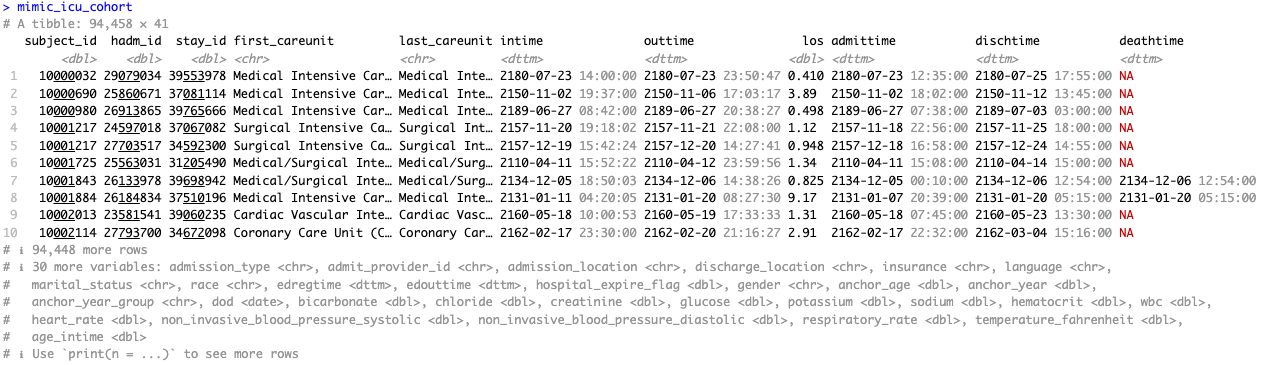
\includegraphics{images/mimic_icu_cohort.png}

\begin{center}\rule{0.5\linewidth}{0.5pt}\end{center}

Solution:

\begin{Shaded}
\begin{Highlighting}[]
\CommentTok{\# Connect to DuckDB}
\NormalTok{con }\OtherTok{\textless{}{-}} \FunctionTok{dbConnect}\NormalTok{(duckdb}\SpecialCharTok{::}\FunctionTok{duckdb}\NormalTok{(), }\AttributeTok{dbdir =} \StringTok{":memory:"}\NormalTok{)}

\CommentTok{\# Write data into DuckDB}
\FunctionTok{dbWriteTable}\NormalTok{(con, }\StringTok{"icustays\_tble"}\NormalTok{, icustays\_tble, }\AttributeTok{overwrite =} \ConstantTok{TRUE}\NormalTok{)}
\FunctionTok{dbWriteTable}\NormalTok{(con, }\StringTok{"admissions\_tble"}\NormalTok{, admissions\_tble, }\AttributeTok{overwrite =} \ConstantTok{TRUE}\NormalTok{)}
\FunctionTok{dbWriteTable}\NormalTok{(con, }\StringTok{"patients\_tble"}\NormalTok{, patients\_tble, }\AttributeTok{overwrite =} \ConstantTok{TRUE}\NormalTok{)}

\CommentTok{\# Load ICU stays data}
\NormalTok{icustays\_tble }\OtherTok{\textless{}{-}} \FunctionTok{dbGetQuery}\NormalTok{(con, }\StringTok{"SELECT * FROM icustays\_tble"}\NormalTok{)}

\CommentTok{\# Load admissions data}
\NormalTok{admissions\_tble }\OtherTok{\textless{}{-}} \FunctionTok{dbGetQuery}\NormalTok{(con, }\StringTok{"SELECT * FROM admissions\_tble"}\NormalTok{)}

\CommentTok{\# Load patients data}
\NormalTok{patients\_tble }\OtherTok{\textless{}{-}} \FunctionTok{dbGetQuery}\NormalTok{(con, }\StringTok{"SELECT * FROM patients\_tble"}\NormalTok{)}
\end{Highlighting}
\end{Shaded}

\begin{Shaded}
\begin{Highlighting}[]
\CommentTok{\# Write data into DuckDB}
\FunctionTok{dbWriteTable}\NormalTok{(con, }\StringTok{"labevents\_tble"}\NormalTok{, labevents\_tble, }\AttributeTok{overwrite =} \ConstantTok{TRUE}\NormalTok{)}
\FunctionTok{dbWriteTable}\NormalTok{(con, }\StringTok{"chartevents\_tble"}\NormalTok{, chartevents\_tble, }\AttributeTok{overwrite =} \ConstantTok{TRUE}\NormalTok{)}

\CommentTok{\# Load lab/chart events}
\NormalTok{labevents\_tble }\OtherTok{\textless{}{-}} \FunctionTok{dbGetQuery}\NormalTok{(con, }\StringTok{"SELECT * FROM labevents\_tble"}\NormalTok{)}
\NormalTok{chartevents\_tble }\OtherTok{\textless{}{-}} \FunctionTok{dbGetQuery}\NormalTok{(con, }\StringTok{"SELECT * FROM chartevents\_tble"}\NormalTok{)}
\end{Highlighting}
\end{Shaded}

\begin{Shaded}
\begin{Highlighting}[]
\CommentTok{\# Merge ICU stays and admissions**}
\NormalTok{mimic\_icu\_cohort }\OtherTok{\textless{}{-}}\NormalTok{ icustays\_tble }\SpecialCharTok{\%\textgreater{}\%}
  \FunctionTok{inner\_join}\NormalTok{(admissions\_tble, }\AttributeTok{by =} \StringTok{"subject\_id"}\NormalTok{) }\SpecialCharTok{\%\textgreater{}\%}
  \FunctionTok{inner\_join}\NormalTok{(patients\_tble, }\AttributeTok{by =} \StringTok{"subject\_id"}\NormalTok{)}
\end{Highlighting}
\end{Shaded}

\begin{verbatim}
Warning in inner_join(., admissions_tble, by = "subject_id"): Detected an unexpected many-to-many relationship between `x` and `y`.
i Row 1 of `x` matches multiple rows in `y`.
i Row 48 of `y` matches multiple rows in `x`.
i If a many-to-many relationship is expected, set `relationship = "many-to-many"` to silence this warning.
\end{verbatim}

\begin{Shaded}
\begin{Highlighting}[]
\CommentTok{\# *Add lab events (most recent lab tests)**}
\NormalTok{mimic\_icu\_cohort }\OtherTok{\textless{}{-}}\NormalTok{ mimic\_icu\_cohort }\SpecialCharTok{\%\textgreater{}\%}
  \FunctionTok{left\_join}\NormalTok{(labevents\_tble, }\AttributeTok{by =} \FunctionTok{c}\NormalTok{(}\StringTok{"subject\_id"}\NormalTok{, }\StringTok{"stay\_id"}\NormalTok{))}
\end{Highlighting}
\end{Shaded}

\begin{Shaded}
\begin{Highlighting}[]
\CommentTok{\# Add chart events (first recorded vital signs)**}
\NormalTok{mimic\_icu\_cohort }\OtherTok{\textless{}{-}}\NormalTok{ mimic\_icu\_cohort }\SpecialCharTok{\%\textgreater{}\%}
  \FunctionTok{left\_join}\NormalTok{(chartevents\_tble, }\AttributeTok{by =} \FunctionTok{c}\NormalTok{(}\StringTok{"subject\_id"}\NormalTok{, }\StringTok{"stay\_id"}\NormalTok{))}

\CommentTok{\#*Ensure each ICU stay corresponds to only one row**}
\NormalTok{mimic\_icu\_cohort }\OtherTok{\textless{}{-}}\NormalTok{ mimic\_icu\_cohort }\SpecialCharTok{\%\textgreater{}\%}
  \FunctionTok{distinct}\NormalTok{(subject\_id, stay\_id, }\AttributeTok{.keep\_all =} \ConstantTok{TRUE}\NormalTok{)}

\CommentTok{\# Sort by subject\_id and stay\_id**}
\NormalTok{mimic\_icu\_cohort }\OtherTok{\textless{}{-}}\NormalTok{ mimic\_icu\_cohort }\SpecialCharTok{\%\textgreater{}\%}
  \FunctionTok{arrange}\NormalTok{(subject\_id, stay\_id)}

\CommentTok{\# Display the final dataset}
\FunctionTok{options}\NormalTok{(}\AttributeTok{width =} \DecValTok{1000}\NormalTok{)}
\FunctionTok{print}\NormalTok{(}\FunctionTok{head}\NormalTok{(mimic\_icu\_cohort, }\DecValTok{10}\NormalTok{))}
\end{Highlighting}
\end{Shaded}

\begin{verbatim}
   subject_id hadm_id.x  stay_id                                   first_careunit                                    last_careunit              intime             outtime       los hadm_id.y           admittime           dischtime deathtime    admission_type admit_provider_id     admission_location       discharge_location insurance language marital_status                   race           edregtime           edouttime hospital_expire_flag admission_hour admission_minute length_of_stay gender anchor_age anchor_year anchor_year_group        dod bicarbonate chloride creatinine glucose potassium sodium hematocrit  wbc heart_rate non-invasive_blood_pressure_diastolic non-invasive_blood_pressure_systolic respiratory_rate temperature_fahrenheit
1    10000032  29079034 39553978               Medical Intensive Care Unit (MICU)               Medical Intensive Care Unit (MICU) 2180-07-23 14:00:00 2180-07-23 23:50:47 0.4102662  22595853 2180-05-06 22:23:00 2180-05-07 17:15:00      <NA>            URGENT            P49AFC TRANSFER FROM HOSPITAL                     HOME  Medicaid  English        WIDOWED                  WHITE 2180-05-06 19:17:00 2180-05-06 23:30:00                    0             22               23      0.7861111      F         52        2180       2014 - 2016 2180-09-09          25       95        0.7     102       6.7    126       41.1  6.9      91.00                                 48.00                                 84.0            24.00                   98.7
2    10000690  25860671 37081114               Medical Intensive Care Unit (MICU)               Medical Intensive Care Unit (MICU) 2150-11-02 19:37:00 2150-11-06 17:03:17 3.8932523  23280645 2150-09-16 19:48:00 2150-09-24 13:50:00      <NA>          EW EMER.            P941QM         EMERGENCY ROOM SKILLED NURSING FACILITY  Medicare  English        WIDOWED                  WHITE 2150-09-16 16:00:00 2150-09-16 21:03:00                    0             19               48      7.7513889      F         86        2150       2008 - 2010 2152-01-30          26      100        1.0      85       4.8    137       36.1  7.1      78.00                                 56.50                                106.0            24.33                   97.7
3    10000980  26913865 39765666               Medical Intensive Care Unit (MICU)               Medical Intensive Care Unit (MICU) 2189-06-27 08:42:00 2189-06-27 20:38:27 0.4975347  20897796 2193-08-15 01:01:00 2193-08-17 15:07:00      <NA> OBSERVATION ADMIT            P55EL5  WALK-IN/SELF REFERRAL         HOME HEALTH CARE  Medicare  English        MARRIED BLACK/AFRICAN AMERICAN 2193-08-14 21:25:00 2193-08-15 02:22:00                    0              1                1      2.5875000      F         73        2186       2008 - 2010 2193-08-26          21      109        2.3      89       3.9    144       27.3  5.3      76.00                                102.00                                154.0            23.50                   98.0
4    10001217  27703517 34592300              Surgical Intensive Care Unit (SICU)              Surgical Intensive Care Unit (SICU) 2157-12-19 15:42:24 2157-12-20 14:27:41 0.9481134  24597018 2157-11-18 22:56:00 2157-11-25 18:00:00      <NA>          EW EMER.            P3610N         EMERGENCY ROOM         HOME HEALTH CARE   Private    Other        MARRIED                  WHITE 2157-11-18 17:38:00 2157-11-19 01:24:00                    0             22               56      6.7944444      F         55        2157       2011 - 2013       <NA>          30      104        0.5      87       4.1    142       37.4  5.4      79.33                                 93.33                                156.0            14.00                   97.6
5    10001217  24597018 37067082              Surgical Intensive Care Unit (SICU)              Surgical Intensive Care Unit (SICU) 2157-11-20 19:18:02 2157-11-21 22:08:00 1.1180324  24597018 2157-11-18 22:56:00 2157-11-25 18:00:00      <NA>          EW EMER.            P3610N         EMERGENCY ROOM         HOME HEALTH CARE   Private    Other        MARRIED                  WHITE 2157-11-18 17:38:00 2157-11-19 01:24:00                    0             22               56      6.7944444      F         55        2157       2011 - 2013       <NA>          22      108        0.6     112       4.2    142       38.1 15.7      86.00                                 90.00                                151.0            18.00                   98.5
6    10001725  25563031 31205490 Medical/Surgical Intensive Care Unit (MICU/SICU) Medical/Surgical Intensive Care Unit (MICU/SICU) 2110-04-11 15:52:22 2110-04-12 23:59:56 1.3385880  25563031 2110-04-11 15:08:00 2110-04-14 15:00:00      <NA>          EW EMER.            P32W56                   PACU                     HOME   Private  English        MARRIED                  WHITE                <NA>                <NA>                    0             15                8      2.9944444      F         46        2110       2011 - 2013       <NA>          NA       98         NA      NA       4.1    139         NA   NA      86.00                                 56.00                                 73.0            19.00                   97.7
7    10001843  26133978 39698942 Medical/Surgical Intensive Care Unit (MICU/SICU) Medical/Surgical Intensive Care Unit (MICU/SICU) 2134-12-05 18:50:03 2134-12-06 14:38:26 0.8252662  21728396 2131-11-09 16:05:00 2131-11-11 11:23:00      <NA> OBSERVATION ADMIT            P32VJE TRANSFER FROM HOSPITAL         HOME HEALTH CARE  Medicare  English         SINGLE                  WHITE                <NA>                <NA>                    0             16                5      1.8041667      M         73        2131       2017 - 2019 2134-12-06          28       97        1.3     131       3.9    138       31.4 10.4     124.50                                 78.00                                110.0            16.50                   97.9
8    10001884  26184834 37510196               Medical Intensive Care Unit (MICU)               Medical Intensive Care Unit (MICU) 2131-01-11 04:20:05 2131-01-20 08:27:30 9.1718171  21192799 2130-10-05 20:04:00 2130-10-06 15:05:00      <NA>    EU OBSERVATION            P99AKB         EMERGENCY ROOM                     <NA>  Medicare  English        MARRIED BLACK/AFRICAN AMERICAN 2130-10-05 11:58:00 2130-10-06 15:05:00                    0             20                4      0.7923611      F         68        2122       2008 - 2010 2131-01-20          30       88        1.1     141       4.5    130       39.7 12.2      49.00                                 30.50                                173.5            13.00                   98.1
9    10002013  23581541 39060235     Cardiac Vascular Intensive Care Unit (CVICU)     Cardiac Vascular Intensive Care Unit (CVICU) 2160-05-18 10:00:53 2160-05-19 17:33:33 1.3143519  21516558 2169-12-03 14:12:00 2169-12-05 17:00:00      <NA> OBSERVATION ADMIT            P11I4S  WALK-IN/SELF REFERRAL         HOME HEALTH CARE  Medicaid  English         SINGLE                  WHITE 2169-12-02 19:30:00 2169-12-03 21:13:00                    0             14               12      2.1166667      F         53        2156       2008 - 2010       <NA>          24      102        0.9     288       3.5    137       34.9  7.2      80.00                                 62.00                                 98.5            14.00                   97.2
10   10002114  27793700 34672098                         Coronary Care Unit (CCU)                         Coronary Care Unit (CCU) 2162-02-17 23:30:00 2162-02-20 21:16:27 2.9072569  27793700 2162-02-17 22:32:00 2162-03-04 15:16:00      <NA> OBSERVATION ADMIT            P46834     PHYSICIAN REFERRAL         HOME HEALTH CARE  Medicaid  English           <NA>                UNKNOWN 2162-02-17 19:35:00 2162-02-17 23:30:00                    0             22               32     14.6972222      M         56        2162       2020 - 2022 2162-12-11          18       NA        3.1      95       6.5    125       34.3 16.8     110.50                                 80.00                                112.0            21.00                   97.9
\end{verbatim}

\begin{Shaded}
\begin{Highlighting}[]
\CommentTok{\# Disconnect from the database}
\FunctionTok{dbDisconnect}\NormalTok{(con, }\AttributeTok{shutdown =} \ConstantTok{TRUE}\NormalTok{)}
\FunctionTok{gc}\NormalTok{()}
\end{Highlighting}
\end{Shaded}

\begin{verbatim}
           used  (Mb) gc trigger  (Mb) max used  (Mb)
Ncells  1956144 104.5    3896008 208.1  3896008 208.1
Vcells 24276776 185.3   74197150 566.1 83584938 637.8
\end{verbatim}

\begin{Shaded}
\begin{Highlighting}[]
\FunctionTok{rm}\NormalTok{(admissions\_tble,duckdb\_table\_icustays,patients\_tble)}
\end{Highlighting}
\end{Shaded}

\begin{verbatim}
Warning in rm(admissions_tble, duckdb_table_icustays, patients_tble): object 'duckdb_table_icustays' not found
\end{verbatim}

\begin{Shaded}
\begin{Highlighting}[]
\FunctionTok{rm}\NormalTok{(base\_shapes,patient\_id,final\_shapes,}
\NormalTok{   itemid\_labels,itemid\_mapping,desired\_order,}
\NormalTok{   extra\_shapes)}

\FunctionTok{rm}\NormalTok{(icustays\_tble,labevents\_tble,chartevents\_tble)}
\end{Highlighting}
\end{Shaded}

\hypertarget{q8.-exploratory-data-analysis-eda}{%
\subsection{Q8. Exploratory data analysis
(EDA)}\label{q8.-exploratory-data-analysis-eda}}

Summarize the following information about the ICU stay cohort
\texttt{mimic\_icu\_cohort} using appropriate numerics or graphs:

\begin{itemize}
\item
  Length of ICU stay \texttt{los} vs demographic variables (race,
  insurance, marital\_status, gender, age at intime)
\item
  Length of ICU stay \texttt{los} vs the last available lab measurements
  before ICU stay
\item
  Length of ICU stay \texttt{los} vs the first vital measurements within
  the ICU stay
\item
  Length of ICU stay \texttt{los} vs first ICU unit
\end{itemize}

\begin{center}\rule{0.5\linewidth}{0.5pt}\end{center}

Solution:

\hypertarget{length-of-icu-stay-los-vs-demographic-variables-race-insurance-marital_status-gender-age-at-intime}{%
\paragraph{\texorpdfstring{Length of ICU stay \texttt{los} vs
demographic variables (race, insurance, marital\_status, gender, age at
intime)}{Length of ICU stay los vs demographic variables (race, insurance, marital\_status, gender, age at intime)}}\label{length-of-icu-stay-los-vs-demographic-variables-race-insurance-marital_status-gender-age-at-intime}}

\begin{Shaded}
\begin{Highlighting}[]
\CommentTok{\# LOS vs Gender}
\CommentTok{\# Remove extreme outliers for better visualization (e.g., focus on LOS \textless{} 50 days)}
\NormalTok{mimic\_icu\_cohort\_filtered }\OtherTok{\textless{}{-}}\NormalTok{ mimic\_icu\_cohort }\SpecialCharTok{\%\textgreater{}\%}
  \FunctionTok{filter}\NormalTok{(los }\SpecialCharTok{\textless{}} \FunctionTok{quantile}\NormalTok{(los, }\FloatTok{0.99}\NormalTok{, }\AttributeTok{na.rm =} \ConstantTok{TRUE}\NormalTok{))  }\CommentTok{\# Remove top 1\% outliers}

\CommentTok{\# Calculate median LOS per race and order the factor levels}
\NormalTok{race\_order }\OtherTok{\textless{}{-}}\NormalTok{ mimic\_icu\_cohort\_filtered }\SpecialCharTok{\%\textgreater{}\%}
  \FunctionTok{group\_by}\NormalTok{(race) }\SpecialCharTok{\%\textgreater{}\%}
  \FunctionTok{summarise}\NormalTok{(}\AttributeTok{median\_los =} \FunctionTok{median}\NormalTok{(los, }\AttributeTok{na.rm =} \ConstantTok{TRUE}\NormalTok{)) }\SpecialCharTok{\%\textgreater{}\%}
  \FunctionTok{arrange}\NormalTok{(median\_los) }\SpecialCharTok{\%\textgreater{}\%}
  \FunctionTok{pull}\NormalTok{(race)}

\NormalTok{mimic\_icu\_cohort\_filtered}\SpecialCharTok{$}\NormalTok{race }\OtherTok{\textless{}{-}} \FunctionTok{factor}\NormalTok{(mimic\_icu\_cohort\_filtered}\SpecialCharTok{$}\NormalTok{race, }
                                         \AttributeTok{levels =}\NormalTok{ race\_order)}

\CommentTok{\# Improved boxplot with better visibility}
\FunctionTok{ggplot}\NormalTok{(mimic\_icu\_cohort\_filtered, }\FunctionTok{aes}\NormalTok{(}\AttributeTok{x =}\NormalTok{ race, }\AttributeTok{y =}\NormalTok{ los, }\AttributeTok{fill =}\NormalTok{ race)) }\SpecialCharTok{+}
  \FunctionTok{geom\_boxplot}\NormalTok{(}\AttributeTok{outlier.shape =} \ConstantTok{NA}\NormalTok{, }\AttributeTok{alpha =} \FloatTok{0.7}\NormalTok{) }\SpecialCharTok{+}  
  \CommentTok{\# Reduce opacity for better visibility}
  \FunctionTok{coord\_flip}\NormalTok{() }\SpecialCharTok{+}  \CommentTok{\# Flip to horizontal for better readability}
  \FunctionTok{theme\_minimal}\NormalTok{() }\SpecialCharTok{+}  \CommentTok{\# Cleaner theme}
  \FunctionTok{theme}\NormalTok{(}
    \AttributeTok{axis.text.y =} \FunctionTok{element\_text}\NormalTok{(}\AttributeTok{size =} \DecValTok{10}\NormalTok{, }\AttributeTok{face =} \StringTok{"bold"}\NormalTok{),  }\CommentTok{\# Bigger labels}
    \AttributeTok{legend.position =} \StringTok{"none"}  \CommentTok{\# Hide legend to declutter}
\NormalTok{  ) }\SpecialCharTok{+}
  \FunctionTok{labs}\NormalTok{(}
    \AttributeTok{title =} \StringTok{"ICU Length of Stay by Race (Filtered Outliers)"}\NormalTok{,}
    \AttributeTok{x =} \StringTok{"Race"}\NormalTok{,}
    \AttributeTok{y =} \StringTok{"Length of Stay (days)"}
\NormalTok{  )}
\end{Highlighting}
\end{Shaded}

\begin{figure}[H]

{\centering 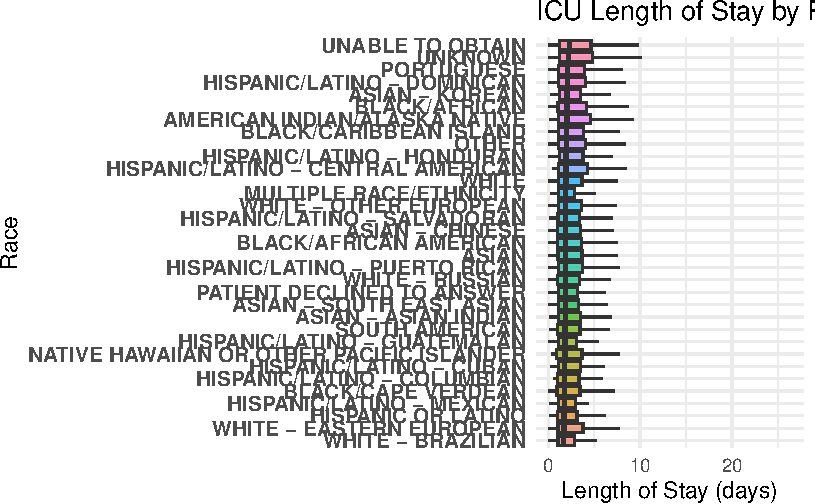
\includegraphics{hw3_files/figure-pdf/8.1-1.pdf}

}

\end{figure}

\begin{Shaded}
\begin{Highlighting}[]
\CommentTok{\# LOS vs Gender}
\CommentTok{\# Improved boxplot + jitter}
\FunctionTok{ggplot}\NormalTok{(mimic\_icu\_cohort\_filtered, }\FunctionTok{aes}\NormalTok{(}\AttributeTok{x =}\NormalTok{ gender, }\AttributeTok{y =}\NormalTok{ los, }
                                      \AttributeTok{fill =}\NormalTok{ gender)) }\SpecialCharTok{+}
  \FunctionTok{geom\_boxplot}\NormalTok{(}\AttributeTok{outlier.shape =} \ConstantTok{NA}\NormalTok{, }\AttributeTok{alpha =} \FloatTok{0.7}\NormalTok{, }\AttributeTok{width =} \FloatTok{0.5}\NormalTok{) }\SpecialCharTok{+}  
  \CommentTok{\# Hide extreme outliers, adjust width}
  \FunctionTok{geom\_jitter}\NormalTok{(}\AttributeTok{width =} \FloatTok{0.15}\NormalTok{, }\AttributeTok{alpha =} \FloatTok{0.05}\NormalTok{, }\AttributeTok{size =} \FloatTok{1.2}\NormalTok{, }
              \AttributeTok{color =} \StringTok{"blue"}\NormalTok{) }\SpecialCharTok{+}  \CommentTok{\# More transparency, smaller points}
  \FunctionTok{theme\_minimal}\NormalTok{() }\SpecialCharTok{+}
  \FunctionTok{labs}\NormalTok{(}\AttributeTok{title =} \StringTok{"ICU Length of Stay by Gender"}\NormalTok{, }\AttributeTok{x =} \StringTok{"Gender"}\NormalTok{, }
       \AttributeTok{y =} \StringTok{"Length of Stay (days)"}\NormalTok{) }\SpecialCharTok{+}
  \FunctionTok{scale\_fill\_manual}\NormalTok{(}\AttributeTok{values =} \FunctionTok{c}\NormalTok{(}\StringTok{"F"} \OtherTok{=} \StringTok{"lightcoral"}\NormalTok{, }\StringTok{"M"} \OtherTok{=} \StringTok{"steelblue"}\NormalTok{)) }\SpecialCharTok{+}  
  \FunctionTok{theme}\NormalTok{(}\AttributeTok{legend.position =} \StringTok{"none"}\NormalTok{)}
\end{Highlighting}
\end{Shaded}

\begin{figure}[H]

{\centering \includegraphics{hw3_files/figure-pdf/8.2-1.pdf}

}

\end{figure}

\begin{Shaded}
\begin{Highlighting}[]
\CommentTok{\# Alternative: Violin plot for better visualization}
\FunctionTok{ggplot}\NormalTok{(mimic\_icu\_cohort\_filtered, }\FunctionTok{aes}\NormalTok{(}\AttributeTok{x =}\NormalTok{ gender, }\AttributeTok{y =}\NormalTok{ los, }\AttributeTok{fill =}\NormalTok{ gender)) }\SpecialCharTok{+}
  \FunctionTok{geom\_violin}\NormalTok{(}\AttributeTok{alpha =} \FloatTok{0.6}\NormalTok{, }\AttributeTok{trim =} \ConstantTok{TRUE}\NormalTok{) }\SpecialCharTok{+}  \CommentTok{\# Smooth density distribution}
  \FunctionTok{geom\_boxplot}\NormalTok{(}\AttributeTok{width =} \FloatTok{0.2}\NormalTok{, }\AttributeTok{fill =} \StringTok{"white"}\NormalTok{, }\AttributeTok{outlier.shape =} \ConstantTok{NA}\NormalTok{) }\SpecialCharTok{+}  
  \CommentTok{\# Overlay boxplot inside violin}
  \FunctionTok{theme\_minimal}\NormalTok{() }\SpecialCharTok{+}
  \FunctionTok{labs}\NormalTok{(}\AttributeTok{title =} \StringTok{"ICU Length of Stay by Gender (Violin + Boxplot)"}\NormalTok{, }
       \AttributeTok{x =} \StringTok{"Gender"}\NormalTok{, }\AttributeTok{y =} \StringTok{"Length of Stay (days)"}\NormalTok{) }\SpecialCharTok{+}
  \FunctionTok{scale\_fill\_manual}\NormalTok{(}\AttributeTok{values =} \FunctionTok{c}\NormalTok{(}\StringTok{"F"} \OtherTok{=} \StringTok{"lightcoral"}\NormalTok{, }\StringTok{"M"} \OtherTok{=} \StringTok{"steelblue"}\NormalTok{)) }\SpecialCharTok{+}  
  \FunctionTok{theme}\NormalTok{(}\AttributeTok{legend.position =} \StringTok{"none"}\NormalTok{)}
\end{Highlighting}
\end{Shaded}

\begin{figure}[H]

{\centering 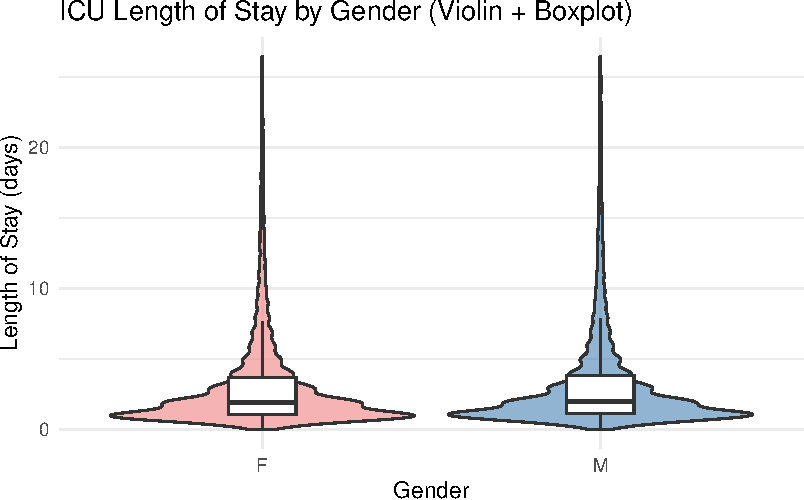
\includegraphics{hw3_files/figure-pdf/8.2-2.pdf}

}

\end{figure}

Most ICU stays are relatively short, with patients mainly concentrated
at the bottom, while the slender tail indicates that a small number of
patients have abnormally prolonged ICU stays. The distribution shapes of
the two genders are similar, indicating that the hospitalization time
patterns of males and females in the ICU are basically the same, with no
significant gender differences.

\begin{Shaded}
\begin{Highlighting}[]
\CommentTok{\# LOS vs Insurance}
\FunctionTok{ggplot}\NormalTok{(mimic\_icu\_cohort\_filtered, }\FunctionTok{aes}\NormalTok{(}\AttributeTok{x =} \FunctionTok{reorder}\NormalTok{(insurance, }
\NormalTok{                                                  los, median, }\AttributeTok{na.rm =} \ConstantTok{TRUE}\NormalTok{), }
                                      \AttributeTok{y =}\NormalTok{ los, }\AttributeTok{fill =}\NormalTok{ insurance)) }\SpecialCharTok{+}
  \FunctionTok{geom\_boxplot}\NormalTok{(}\AttributeTok{outlier.shape =} \ConstantTok{NA}\NormalTok{, }\AttributeTok{alpha =} \FloatTok{0.7}\NormalTok{) }\SpecialCharTok{+}
  \FunctionTok{coord\_flip}\NormalTok{() }\SpecialCharTok{+}
  \FunctionTok{theme\_minimal}\NormalTok{() }\SpecialCharTok{+}
  \FunctionTok{labs}\NormalTok{(}\AttributeTok{title =} \StringTok{"ICU Length of Stay by Insurance"}\NormalTok{, }
       \AttributeTok{x =} \StringTok{"Insurance Type"}\NormalTok{, }\AttributeTok{y =} \StringTok{"Length of Stay (days)"}\NormalTok{) }\SpecialCharTok{+}
  \FunctionTok{theme}\NormalTok{(}\AttributeTok{legend.position =} \StringTok{"none"}\NormalTok{)}
\end{Highlighting}
\end{Shaded}

\begin{figure}[H]

{\centering 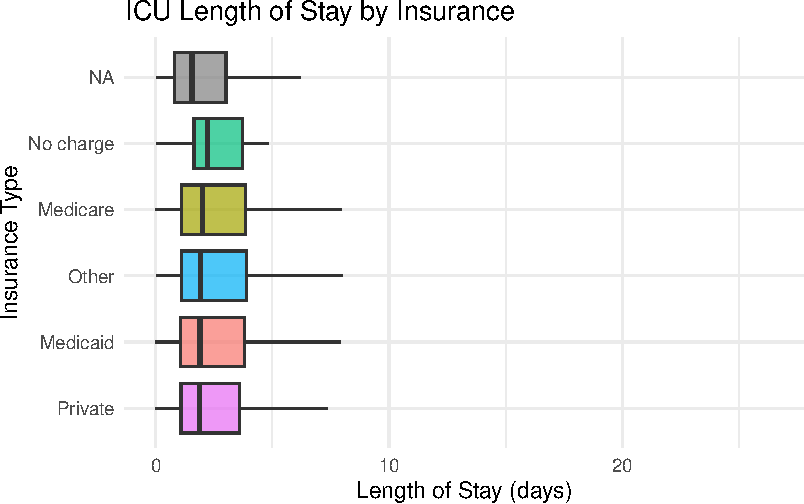
\includegraphics{hw3_files/figure-pdf/8.3-1.pdf}

}

\end{figure}

\begin{Shaded}
\begin{Highlighting}[]
\CommentTok{\# LOS vs Marital Status}
\FunctionTok{ggplot}\NormalTok{(mimic\_icu\_cohort\_filtered, }\FunctionTok{aes}\NormalTok{(}\AttributeTok{x =} \FunctionTok{reorder}\NormalTok{(marital\_status, los, }
\NormalTok{                                                  median, }\AttributeTok{na.rm =} \ConstantTok{TRUE}\NormalTok{), }
                                      \AttributeTok{y =}\NormalTok{ los, }\AttributeTok{fill =}\NormalTok{ marital\_status)) }\SpecialCharTok{+}
  \FunctionTok{geom\_boxplot}\NormalTok{(}\AttributeTok{outlier.shape =} \ConstantTok{NA}\NormalTok{, }\AttributeTok{alpha =} \FloatTok{0.7}\NormalTok{) }\SpecialCharTok{+}
  \FunctionTok{coord\_flip}\NormalTok{() }\SpecialCharTok{+}
  \FunctionTok{theme\_minimal}\NormalTok{() }\SpecialCharTok{+}
  \FunctionTok{labs}\NormalTok{(}\AttributeTok{title =} \StringTok{"ICU Length of Stay by Marital Status"}\NormalTok{, }\AttributeTok{x =} \StringTok{"Marital Status"}\NormalTok{, }
       \AttributeTok{y =} \StringTok{"Length of Stay (days)"}\NormalTok{) }\SpecialCharTok{+}
  \FunctionTok{theme}\NormalTok{(}\AttributeTok{legend.position =} \StringTok{"none"}\NormalTok{)}
\end{Highlighting}
\end{Shaded}

\begin{figure}[H]

{\centering 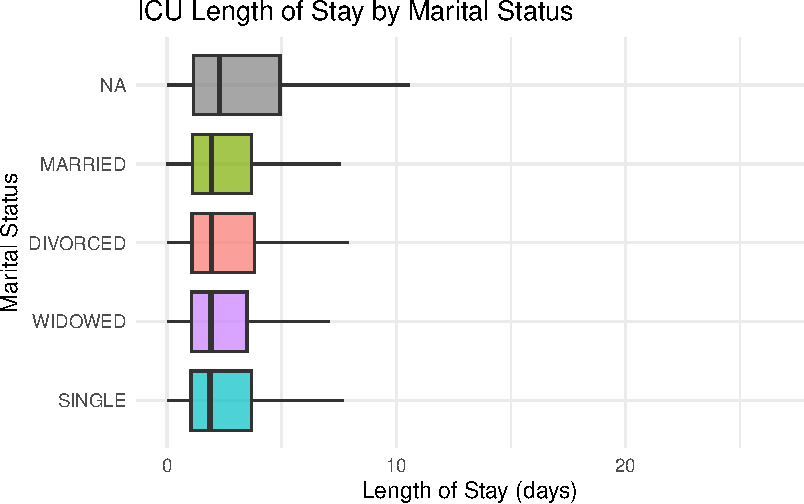
\includegraphics{hw3_files/figure-pdf/8.4-1.pdf}

}

\end{figure}

\begin{Shaded}
\begin{Highlighting}[]
\CommentTok{\# Scatterplot: LOS vs Age}
\FunctionTok{ggplot}\NormalTok{(mimic\_icu\_cohort\_filtered, }\FunctionTok{aes}\NormalTok{(}\AttributeTok{x =}\NormalTok{ anchor\_age, }\AttributeTok{y =}\NormalTok{ los)) }\SpecialCharTok{+}
  \FunctionTok{geom\_point}\NormalTok{(}\AttributeTok{alpha =} \FloatTok{0.2}\NormalTok{, }\AttributeTok{color =} \StringTok{"blue"}\NormalTok{, }\AttributeTok{size =} \FloatTok{0.8}\NormalTok{) }\SpecialCharTok{+}  
  \FunctionTok{geom\_smooth}\NormalTok{(}\AttributeTok{method =} \StringTok{"loess"}\NormalTok{, }\AttributeTok{color =} \StringTok{"red"}\NormalTok{, }\AttributeTok{se =} \ConstantTok{TRUE}\NormalTok{) }\SpecialCharTok{+}
  \FunctionTok{theme\_minimal}\NormalTok{() }\SpecialCharTok{+}
  \FunctionTok{labs}\NormalTok{(}\AttributeTok{title =} \StringTok{"ICU Length of Stay vs Age"}\NormalTok{, }\AttributeTok{x =} \StringTok{"Age at Admission"}\NormalTok{, }
       \AttributeTok{y =} \StringTok{"Length of Stay (days)"}\NormalTok{) }\SpecialCharTok{+}
  \FunctionTok{scale\_y\_continuous}\NormalTok{(}\AttributeTok{limits =} \FunctionTok{c}\NormalTok{(}\DecValTok{0}\NormalTok{, }\DecValTok{50}\NormalTok{))  }
\end{Highlighting}
\end{Shaded}

\begin{verbatim}
`geom_smooth()` using formula = 'y ~ x'
\end{verbatim}

\begin{verbatim}
Warning: Failed to fit group -1.
Caused by error in `predLoess()`:
! workspace required (13114052915) is too large probably because of setting 'se = TRUE'.
\end{verbatim}

\begin{figure}[H]

{\centering \includegraphics{hw3_files/figure-pdf/8.5-1.pdf}

}

\end{figure}

\hypertarget{length-of-icu-stay-los-vs-the-last-available-lab-measurements-before-icu-stay}{%
\paragraph{Length of ICU stay los vs the last available lab measurements
before ICU
stay}\label{length-of-icu-stay-los-vs-the-last-available-lab-measurements-before-icu-stay}}

\begin{Shaded}
\begin{Highlighting}[]
\CommentTok{\# Convert from wide format to long format}
\NormalTok{mimic\_icu\_long }\OtherTok{\textless{}{-}}\NormalTok{ mimic\_icu\_cohort\_filtered }\SpecialCharTok{\%\textgreater{}\%}
  \FunctionTok{pivot\_longer}\NormalTok{(}\AttributeTok{cols =} \FunctionTok{c}\NormalTok{(}\StringTok{"bicarbonate"}\NormalTok{, }\StringTok{"chloride"}\NormalTok{, }\StringTok{"creatinine"}\NormalTok{, }\StringTok{"glucose"}\NormalTok{,}
                        \StringTok{"potassium"}\NormalTok{, }\StringTok{"sodium"}\NormalTok{, }\StringTok{"hematocrit"}\NormalTok{, }\StringTok{"wbc"}\NormalTok{),}
               \AttributeTok{names\_to =} \StringTok{"item\_name"}\NormalTok{, }\AttributeTok{values\_to =} \StringTok{"valuenum"}\NormalTok{) }\SpecialCharTok{\%\textgreater{}\%}
  \FunctionTok{filter}\NormalTok{(}\SpecialCharTok{!}\FunctionTok{is.na}\NormalTok{(valuenum) }\SpecialCharTok{\&} \SpecialCharTok{!}\FunctionTok{is.na}\NormalTok{(los))  }\CommentTok{\# Remove missing values}
\end{Highlighting}
\end{Shaded}

\begin{Shaded}
\begin{Highlighting}[]
\CommentTok{\# Sample a smaller subset to improve performance}
\NormalTok{mimic\_icu\_sampled }\OtherTok{\textless{}{-}}\NormalTok{ mimic\_icu\_long }\SpecialCharTok{\%\textgreater{}\%}
  \FunctionTok{slice\_sample}\NormalTok{(}\AttributeTok{n =} \DecValTok{50000}\NormalTok{)  }\CommentTok{\# Adjust this number as needed}

\CommentTok{\# LOS vs Valuenum (Grouped by Lab Test)}
\FunctionTok{ggplot}\NormalTok{(mimic\_icu\_sampled, }\FunctionTok{aes}\NormalTok{(}\AttributeTok{x =}\NormalTok{ valuenum, }\AttributeTok{y =}\NormalTok{ los, }\AttributeTok{color =}\NormalTok{ item\_name)) }\SpecialCharTok{+}
  \FunctionTok{geom\_point}\NormalTok{(}\AttributeTok{alpha =} \FloatTok{0.3}\NormalTok{, }\AttributeTok{size =} \FloatTok{0.5}\NormalTok{) }\SpecialCharTok{+}  
  \FunctionTok{geom\_smooth}\NormalTok{(}\AttributeTok{method =} \StringTok{"loess"}\NormalTok{, }\AttributeTok{se =} \ConstantTok{FALSE}\NormalTok{, }\AttributeTok{linetype =} \StringTok{"dashed"}\NormalTok{) }\SpecialCharTok{+}  
  \FunctionTok{facet\_wrap}\NormalTok{(}\SpecialCharTok{\textasciitilde{}}\NormalTok{ item\_name, }\AttributeTok{scales =} \StringTok{"free\_x"}\NormalTok{) }\SpecialCharTok{+}  \CommentTok{\# Facet by lab test}
  \FunctionTok{theme\_minimal}\NormalTok{() }\SpecialCharTok{+}
  \FunctionTok{labs}\NormalTok{(}\AttributeTok{title =} \StringTok{"ICU LOS vs Last Available Lab Measurements"}\NormalTok{,}
       \AttributeTok{x =} \StringTok{"Lab Measurement (Valuenum)"}\NormalTok{, }\AttributeTok{y =} \StringTok{"Length of ICU Stay (days)"}\NormalTok{, }
       \AttributeTok{color =} \StringTok{"Lab Test"}\NormalTok{) }\SpecialCharTok{+}
  \FunctionTok{theme}\NormalTok{(}\AttributeTok{legend.position =} \StringTok{"none"}\NormalTok{)  }\CommentTok{\# Hide legend if unnecessary}
\end{Highlighting}
\end{Shaded}

\begin{verbatim}
`geom_smooth()` using formula = 'y ~ x'
\end{verbatim}

\begin{figure}[H]

{\centering 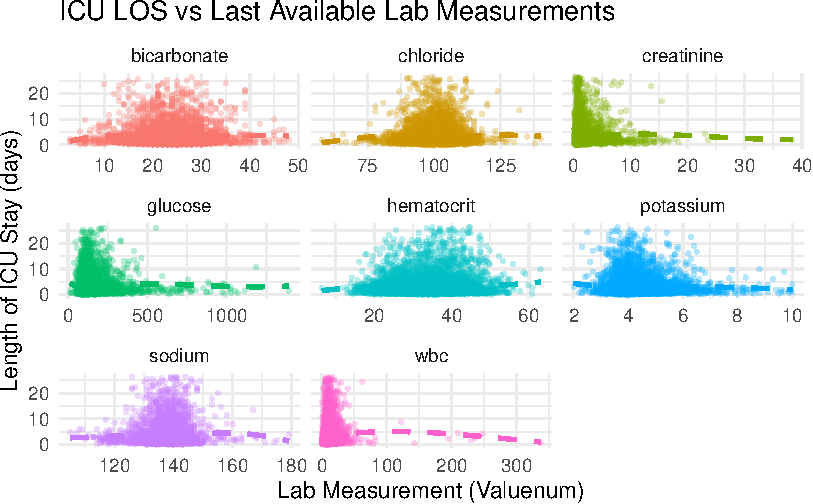
\includegraphics{hw3_files/figure-pdf/unnamed-chunk-41-1.pdf}

}

\end{figure}

\begin{Shaded}
\begin{Highlighting}[]
\FunctionTok{rm}\NormalTok{(mimic\_icu\_long,mimic\_icu\_sampled)}
\end{Highlighting}
\end{Shaded}

\hypertarget{length-of-icu-stay-los-vs-the-first-vital-measurements-within-the-icu-stay}{%
\paragraph{Length of ICU stay los vs the first vital measurements within
the ICU
stay}\label{length-of-icu-stay-los-vs-the-first-vital-measurements-within-the-icu-stay}}

\begin{Shaded}
\begin{Highlighting}[]
\CommentTok{\# Convert from wide format to long format using correct column names}
\NormalTok{mimic\_icu\_long }\OtherTok{\textless{}{-}}\NormalTok{ mimic\_icu\_cohort\_filtered }\SpecialCharTok{\%\textgreater{}\%}
  \FunctionTok{pivot\_longer}\NormalTok{(}\AttributeTok{cols =} \FunctionTok{c}\NormalTok{(}\StringTok{"heart\_rate"}\NormalTok{, }\StringTok{"non{-}invasive\_blood\_pressure\_diastolic"}\NormalTok{, }
                        \StringTok{"non{-}invasive\_blood\_pressure\_systolic"}\NormalTok{, }
                        \StringTok{"respiratory\_rate"}\NormalTok{, }
                        \StringTok{"temperature\_fahrenheit"}\NormalTok{),}
               \AttributeTok{names\_to =} \StringTok{"item\_name"}\NormalTok{, }\AttributeTok{values\_to =} \StringTok{"valuenum"}\NormalTok{) }\SpecialCharTok{\%\textgreater{}\%}
  \FunctionTok{filter}\NormalTok{(}\SpecialCharTok{!}\FunctionTok{is.na}\NormalTok{(valuenum) }\SpecialCharTok{\&} \SpecialCharTok{!}\FunctionTok{is.na}\NormalTok{(los))  }\CommentTok{\# Remove missing values}
\end{Highlighting}
\end{Shaded}

\begin{Shaded}
\begin{Highlighting}[]
\CommentTok{\# Sample a smaller subset to improve performance}
\NormalTok{mimic\_icu\_sampled }\OtherTok{\textless{}{-}}\NormalTok{ mimic\_icu\_long }\SpecialCharTok{\%\textgreater{}\%}
  \FunctionTok{slice\_sample}\NormalTok{(}\AttributeTok{n =} \DecValTok{50000}\NormalTok{)  }\CommentTok{\# Adjust this number as needed}

\CommentTok{\# LOS vs Valuenum (Grouped by Lab Test)}
\FunctionTok{ggplot}\NormalTok{(mimic\_icu\_sampled, }\FunctionTok{aes}\NormalTok{(}\AttributeTok{x =}\NormalTok{ valuenum, }\AttributeTok{y =}\NormalTok{ los, }\AttributeTok{color =}\NormalTok{ item\_name)) }\SpecialCharTok{+}
  \FunctionTok{geom\_point}\NormalTok{(}\AttributeTok{alpha =} \FloatTok{0.5}\NormalTok{) }\SpecialCharTok{+}  \CommentTok{\# Reduce opacity for better visualization}
  \FunctionTok{geom\_smooth}\NormalTok{(}\AttributeTok{method =} \StringTok{"loess"}\NormalTok{, }\AttributeTok{se =} \ConstantTok{FALSE}\NormalTok{, }\AttributeTok{linetype =} \StringTok{"dashed"}\NormalTok{) }\SpecialCharTok{+}  
  \FunctionTok{facet\_wrap}\NormalTok{(}\SpecialCharTok{\textasciitilde{}}\NormalTok{ item\_name, }\AttributeTok{scales =} \StringTok{"free\_x"}\NormalTok{) }\SpecialCharTok{+}  
  \FunctionTok{theme\_minimal}\NormalTok{() }\SpecialCharTok{+}
  \FunctionTok{labs}\NormalTok{(}\AttributeTok{title =} \StringTok{"ICU LOS vs First Vital Measurements"}\NormalTok{,}
       \AttributeTok{x =} \StringTok{"Vital Measurement (Valuenum)"}\NormalTok{, }\AttributeTok{y =} \StringTok{"Length of ICU Stay (days)"}\NormalTok{, }
       \AttributeTok{color =} \StringTok{"Vital Test"}\NormalTok{) }\SpecialCharTok{+}
  \FunctionTok{theme}\NormalTok{(}\AttributeTok{legend.position =} \StringTok{"none"}\NormalTok{)  }\CommentTok{\# Hide redundant legend}
\end{Highlighting}
\end{Shaded}

\begin{verbatim}
`geom_smooth()` using formula = 'y ~ x'
\end{verbatim}

\begin{figure}[H]

{\centering 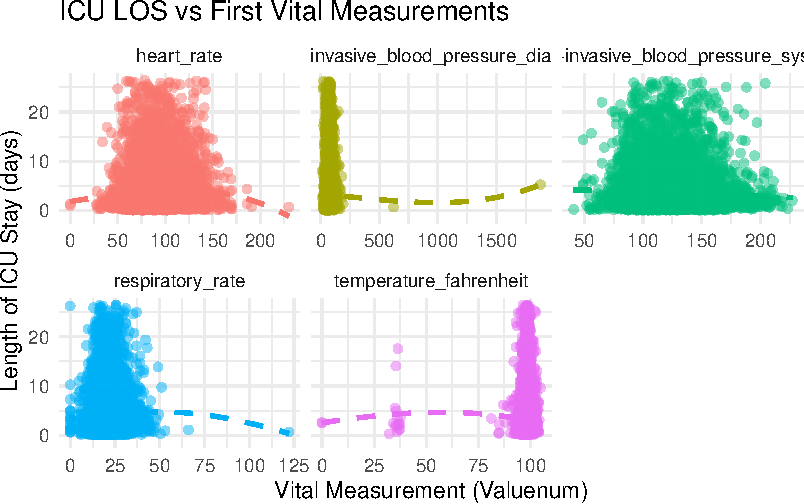
\includegraphics{hw3_files/figure-pdf/8.7-1.pdf}

}

\end{figure}

\begin{Shaded}
\begin{Highlighting}[]
\FunctionTok{rm}\NormalTok{(mimic\_icu\_long,mimic\_icu\_sampled)}
\end{Highlighting}
\end{Shaded}

\hypertarget{length-of-icu-stay-los-vs-first-icu-unit}{%
\paragraph{Length of ICU stay los vs first ICU
unit}\label{length-of-icu-stay-los-vs-first-icu-unit}}

\begin{Shaded}
\begin{Highlighting}[]
\FunctionTok{ggplot}\NormalTok{(mimic\_icu\_cohort\_filtered, }\FunctionTok{aes}\NormalTok{(}\AttributeTok{x =}\NormalTok{ first\_careunit, }\AttributeTok{y =}\NormalTok{ los, }
                                      \AttributeTok{fill =}\NormalTok{ first\_careunit)) }\SpecialCharTok{+}
  \FunctionTok{geom\_boxplot}\NormalTok{(}\AttributeTok{alpha =} \FloatTok{0.7}\NormalTok{, }\AttributeTok{outlier.shape =} \ConstantTok{NA}\NormalTok{) }\SpecialCharTok{+}  \CommentTok{\# Avoid extreme outliers}
  \FunctionTok{theme\_minimal}\NormalTok{() }\SpecialCharTok{+}
  \FunctionTok{labs}\NormalTok{(}\AttributeTok{title =} \StringTok{"ICU LOS vs First ICU Unit"}\NormalTok{,}
       \AttributeTok{x =} \StringTok{"First ICU Unit"}\NormalTok{, }\AttributeTok{y =} \StringTok{"Length of ICU Stay (days)"}\NormalTok{) }\SpecialCharTok{+}
  \FunctionTok{theme}\NormalTok{(}\AttributeTok{axis.text.x =} \FunctionTok{element\_text}\NormalTok{(}\AttributeTok{angle =} \DecValTok{45}\NormalTok{, }\AttributeTok{hjust =} \DecValTok{1}\NormalTok{), }
        \AttributeTok{legend.position =} \StringTok{"none"}\NormalTok{)}
\end{Highlighting}
\end{Shaded}

\begin{figure}[H]

{\centering 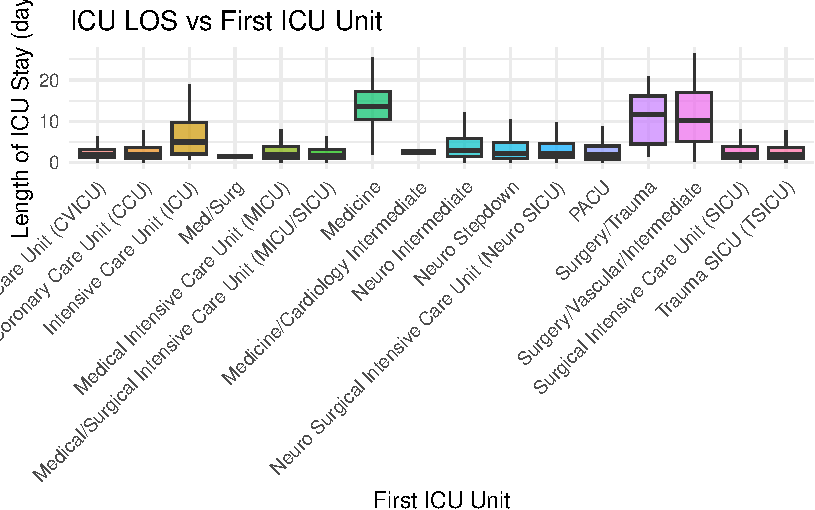
\includegraphics{hw3_files/figure-pdf/unnamed-chunk-43-1.pdf}

}

\end{figure}



\end{document}
